\clearpage

\chapter{Genotype Calling}

\section{Introduction}

Data are now available where individuals have been either sequenced at low coverage, assayed on a genotyping microarray, or both.  Whilst genotypes from the current generation of microarrays are very accurate (greater than 99\% accuracy and call rate)~\citep{Ritchie2011}, it is possible to extract even more accuracy and better call rates for similar computational expense by combining both sources of data. It may be that both sequence and array data are available on all individuals or only a subset of individuals is assayed on both technologies. Ideally both sources of data will be of high quality and agree on the genotypes at a SNP. Genotype arrays tend to produce good data at common SNPs where there is good separation between clusters of allele intensities.  Sequencing data quality improves with sequencing coverage and where the SNP being called is located in a region where read mapping quality is good. In this chapter, we present a model that accommodates both data types and demonstrate its efficacy on recent 1000 Genomes Project data~\citep{Consortium2010,1000G_phase1} .

Genotype calling from arrays will be harder at low frequency SNPs where some clusters have very few (or no) observations as models can be difficult to fit reliably. Where the SNP is monomorphic in the study sample there should only be one cluster. This can be problematic for genotype calling algorithms, as most tend to fit models that assume three clusters of allele intensities exist.  It is also not difficult to find instances of SNPs where clusters are poorly separated, in which case there is significant ambiguity about genotypes that lie at the boundaries between clusters.  

Calling genotypes from sequencing data at low frequency SNPs does not involve a clustering step so in theory is better able to produce accurate calls, given a sufficient number of reads span the SNP being called (sequence coverage). Since cost increases with coverage, datasets that consist of low-coverage sequencing are not uncommon. For example, the 1000 Genomes Project used low-coverage sequencing (approximately 4X per sample) to obtain genome-wide data on its Phase I study samples. If coverage is low then it may be that there is limited information about which individuals carry the rare alleles. It may also be the case that mapping errors lead to false calls in the reads. Such errors can occur at SNPs near indels and while considerable progress has been made to avoid such problems~\citep{lunter2011stampy,li2011improving} they cannot be completely discounted. 

The model we present in this chapter has been designed with these considerations in mind. We jointly model the array and sequence data at each SNP but allow the model to adapt to data quality. So for example, if there is disagreement between the sequence data and the array data at a SNP the model has the flexibility to down weight the set of data with the lower quality. For example, if the sequencing is very good but the array data contains ambiguous observations or poorly separated clusters then the model will tend to exploit the sequence data to ``mop up'' ambiguous array samples and delineate clusters. At rare SNPs it may be that there is partial information in both the sequence and array data so that by fusing these data types together we can improve the calling.

Our method is developed within a Bayesian framework that allows us to use prior information to inform model fit. By extracting information about likely locations of cluster centres from training datasets we have developed useful priors for situations where a genotype cluster has very few observations. In addition, we have analysed how cluster centre positions relate to maximum allele intensities and have developed useful ways to initialise the EM algorithm we use to fit our model. A useful feature of our method is that we can handle data sets where individuals were only assayed on microarrays, have both microarray and sequence data available or only a subset of individuals were sequenced. We investigate the performance of our method and other popular software in these scenarios.

This chapter largely covers the research published in \cite{oconnell2012}.  Our method is implemented in a program named Chiamante which is available online\footnote{\url{http://www.stats.ox.ac.uk/~oconnell/chiamante/}}.


\section{Background}
\subsection{Illumina microarray data}
The Illumina HumanOmni2.5 microarray assays $\approx$ 2.45 million SNPs that were identified in the 1000 Genomes pilot project using Infinium HD assays~\citep{Steemers2006}.  Locus specific 50-mer probes hybridise up to one base before the SNP of interest, a single base extension then labels the allele and two colour fluorescent staining produces a signal intensity for the allele.  Illumina's normalisation routine~\citep{kermani2006artificial} was applied to the raw intensities which aims to make distributions comparable between chips and hence aid genotype calling.  Figure~\ref{chap2:easysnp} (left) shows data for a high quality SNP for 1,525 individuals that are coloured according to genotype assigned by Illumina's standard software.   Various cluster analysis methods (described in the proceeding sub-sections) can then applied to the normalised intensities to convert them into hard genotype calls. Whilst there is good discrimination between genotypes for the vast majority of SNPs, more challenging loci are present which is where the performance of different calling methods can be important. Figure~\ref{chap2:fig:scatterplots} in the results section demonstrates some more difficult loci.


\begin{figure}
  \begin{center} 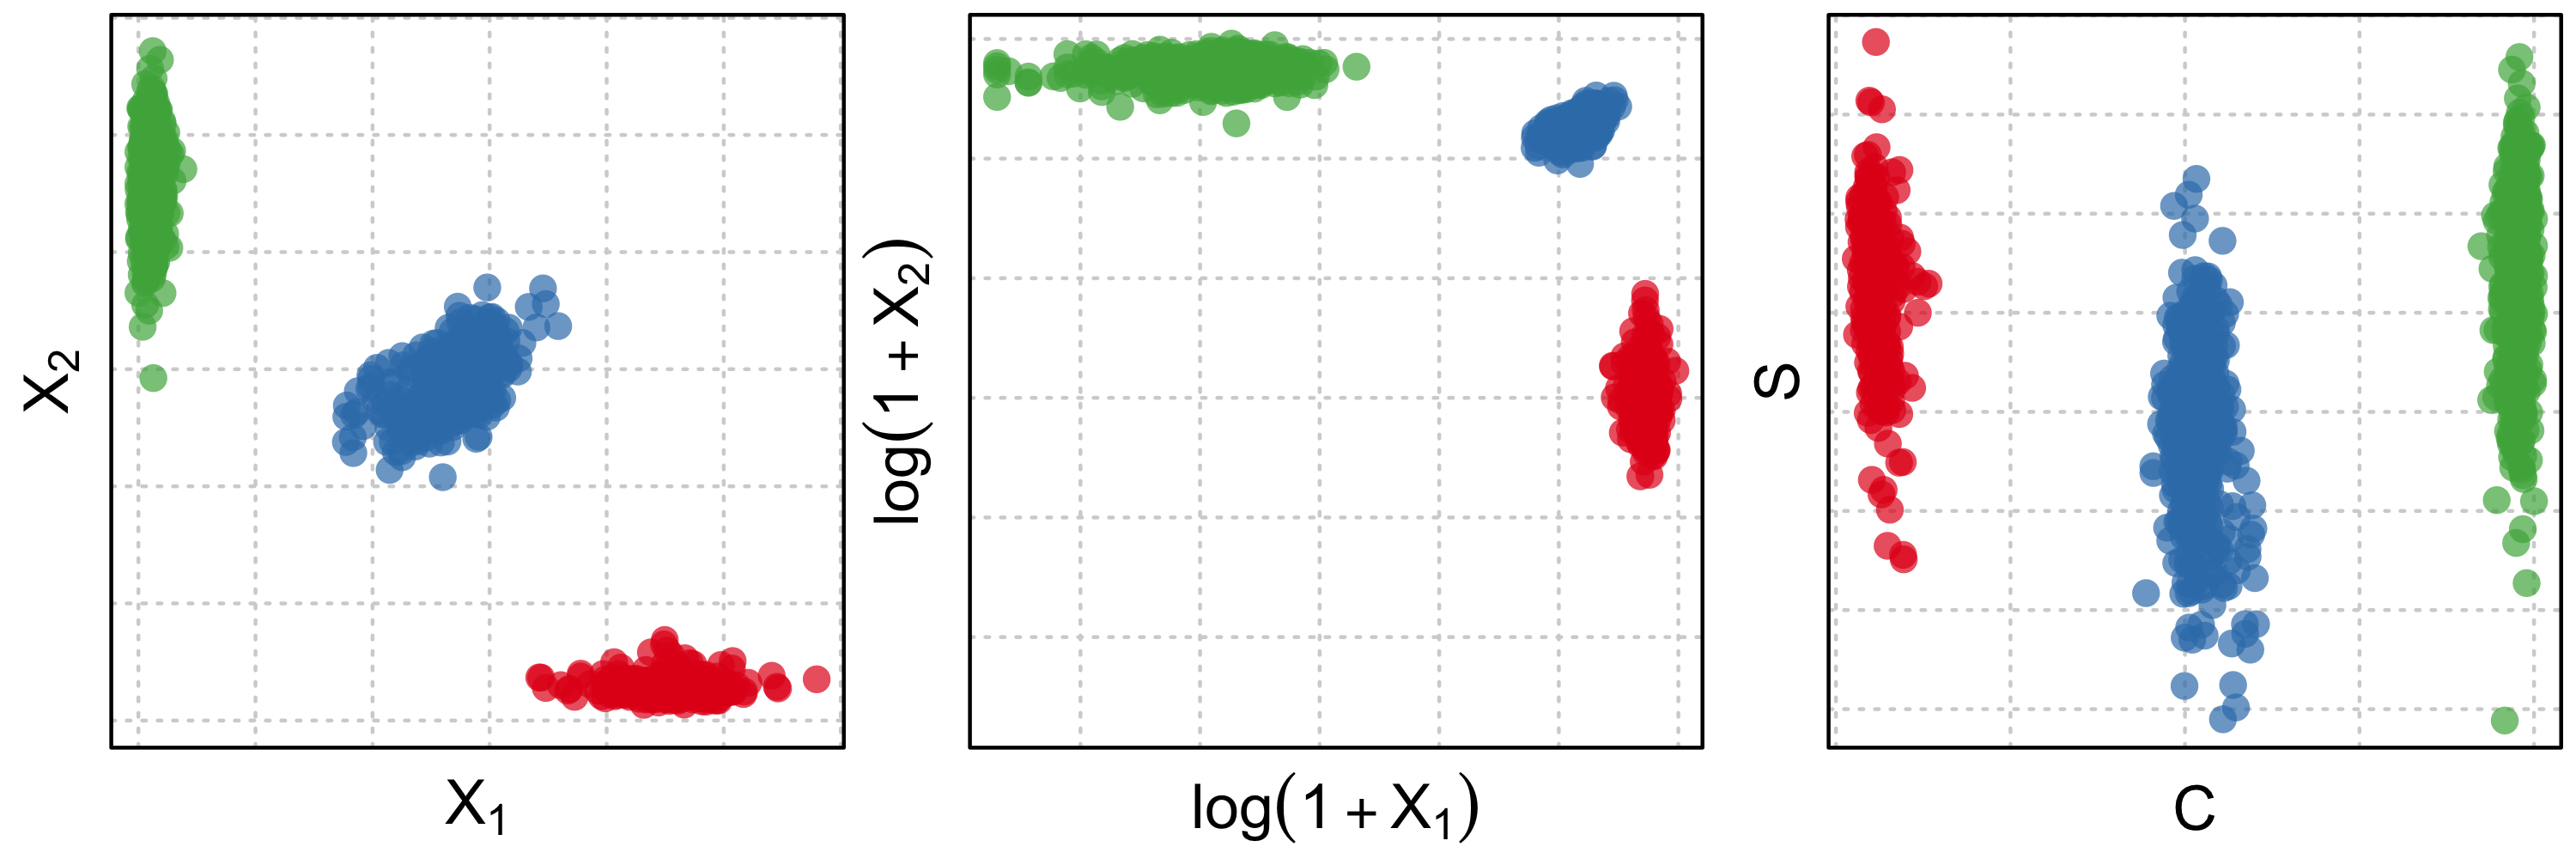
\includegraphics[width=\textwidth]{chap2figs/snpexample_1}
    \caption[Example microarray data from a typical high quality SNP]{Example microarray data from a typical high quality SNP from the Illumina Omni2.5S array assaying 1525 samples. The horizontal axis is the allelic intensity (or a transformation of it) for allele 1, the vertical axis is the intensity of allele 2.  Points are coloured by genotype called by Illumina's genotyping software.  Clusters are well separated and calling genotypes is not problematic. \textbf{Left:} The normalised values. \textbf{Centre:} The $\log$ transformed values which is the scale our algorithm works on. \textbf{Right:} The `strength' $S$ (vertical) and `contrast' $C$ (horizontal) transformations used by the Illuminus algorithm.}
\label{chap2:easysnp}
  \end{center} 
\end{figure}

\subsection{Genotype calling}
Assume we have microarray data on $N$ samples at a bi-allelic SNP as position $l$ and use $G_{il}$ to denote the unobserved genotype of the $i$th sample at this locus. The genotypes $G_{il}$ are the count of the number of non-reference alleles or a missing  value (NULL), that is $G_{il} \in \{0, 1 ,2, \NULL \}$. We use $\{I^1_{il}, I^2_{il}\}$ to denote the normalised bivariate signal intensities of the two alleles (1 and 2) at the SNP. In the following sections, we discard  $i$ or $l$ when we are only describing one particular SNP or individual respectively. The goal of genotype calling is to find the posterior probability of each genotype value given the microarray data, $P(G|I^1,I^2)$. Most methods achieve this via assuming some probability distribution $f_j(I^1,I^2;\theta_j)$ with parameters $\theta_j$ for the array data under genotype $j$, we can then calculate the posterior probability for each genotype via Bayes Rule:
$$P(G=j|I^1,I^2) = \frac{ P(G=j)\times f_j(I^1,I^2;\theta_j) } { \sum_{k=0}^3P(G=k)\times f_k(I^1,I^2;\theta_k) }$$
where $P(G=j)$ is the marginal probability of genotype $j$. We can then take $$\hat{G}=\argmax_jP(G=j|I^1,I^2)$$  as the hard genotype call for individual $i$. Additionally, if the posterior probability does not exceed some threshold we may flag it as missing. Alternatively (and more correctly), these posterior probabilities can be propagated through to other analyses such as phasing, imputation and association testing.

Genotype calling methods differ in three key ways; the choice of of probability distribution for $f_j(I^1,I^2;\theta_j)$, the parameter estimation routine for $\theta_j$ and choice of data transformation. We briefly describe the models and inference used by other methods the next section, we detail our own technique in section~\ref{chap2:chiamante}.

\subsection{Statistical distributions}\label{chap2:statdist}
We define several common statistical distributions that will be used throughout this chapter here.  

The bivariate Gaussian distribution:
$$\phi(X_i;\mu,\Sigma) = (2\pi)^{-d/2} |\Sigma|^{-1/2}\times exp\left(\half (X_i - \mu)^T\Sigma^{-1}(X_i-\mu)\right)$$
where $d=2$, $\mu$ and $\Sigma$ are the dimension, mean and covariance. 

The bivariate \st distribution:
$$s(X_i;\mu,\Sigma,\upsilon) = \frac{\Gamma(\frac{d+\upsilon}{2})}{\Gamma(\upsilon/2)(\upsilon\pi)^{d/2}}|\Sigma|^{-1/2} \times [1+\frac{1}{\upsilon}(X_i - \mu)^T \Sigma^{-1}(X_i - \mu)]^{-(d+\upsilon)/2}$$
where $\upsilon$ are the degrees of freedom.  The \st can be useful (as opposed to a Gaussian) if the data are over dispersed. We can also introduce a latent scale variable $u$ and represent the \st as a scaled mixture of normal distributions 
$$s(X_i;\mu,\Sigma,\upsilon) = \int_0^{\infty} \phi(X_i;\mu,\Sigma / u_i)Gam(u_i|\upsilon/2,\upsilon/2) du$$ where $Gam$ is the pdf of the Gamma distribution:
$$Gam(u_i|,\alpha,\beta) = \frac{\beta^\alpha}{\Gamma(\alpha)} u_i^{\alpha-1}e^{-\beta u_i}$$
This latent variable representation is useful as it allows proper estimation of the covariance matrix via the EM algorithm~\citep{peel2000robust}. This is important for the inference routine we describe in the section~\ref{chap2:inference}. 

%% The Beta distribution:

%% The Beta distribution is a useful prior for parameters that are constrained to be in the range $[0,1]$, for example the probability of success in a Binomial Distribution.


%% $$multinomial$$
%% $$Dirichlet$$

%% $$Inverse-Wishart$$

\section{Existing methods}
\subsection{Illumina's GenTrain2 Algorithm}
Illumina provides a proprietary algorithm (GenTrain) for genotype calling from its genotype microarrays as part of its Genome Studio software, the current version of the software is GenTrain2~\citep{gentrain2}.  In the typical use case, the end-user performs calling using a ``cluster file'' which contains pre-defined cluster centroids for each locus. These centroids were found using HapMap samples where genotypes at each locus are already known from previous assays.  Genotypes on new data are assigned according to which cluster an observation is nearest to. There is no formal description available of exactly what distance measure is used or how these initial clusters are estimated.  Nevertheless, as can be seen the results section the method produces highly accurate calls. We evaluate GenTrain2 calls that were created at the Broad Institute using the standard cluster file for the Omni2.5S chip.  These are available on the 1000 Genomes FTP site \footnote{\url{ftp://ftp.1000genomes.ebi.ac.uk/vol1/ftp/technical/working/20110527_bi_omni_1525_v2_genotypes/}}

\subsection{Illuminus}
Illuminus~\citep{Teo2007} fits a four component mixture of truncated bivariate \st distributions to the ``contrast'' and ``strength'' of the signal intensities at each locus.  Contrast and strength for a given SNP are defined respectively as,
$$C_{i} = \frac{I_i^1 - I_i^2}{I_i^1 + I_i^2}$$
$$S_{i} = \log(I_i^1 + I_i^2)$$
we plot the contrast and strength values for a SNP in Figure~\ref{chap2:easysnp}(right). Posterior probabilities for individual $i$ are found via,
$$P(G_i=j|C_i,S_i) \propto  \lambda_j~t_j(C_i,S_i;\mu_j,\Sigma_j,\upsilon_j)$$
where $\lambda_j$ are the frequencies of the genotypes for $j\in\{0,1,2\}$ constrained to be in Hardy-Weinberg Equilibrium, and $\lambda_{NULL}$ is the proportion of missing data. The density used for observations, $t_j$ is a truncated \st distribution with mean, variance and degrees of freedom equal to  $\mu_j$, $\Sigma_j$ and $\upsilon_j$ respectively;

$$t_0(C,S;\mu_0,\Sigma_0,\upsilon_0) = \frac{s(C,S;\mu_0,\Sigma_0,\upsilon_0)}{1-\int^{-1}_{-\infty} s(C,S;\mu_0,\Sigma_0,\upsilon_0) \textrm{d}C } $$

$$t_1(C,S;\mu_1,\Sigma_1,\upsilon_1) = \frac{s(C,S;\mu_1,\Sigma_1,\upsilon_1)}{\int^{1}_{-1} s(C,S;\mu_1,\Sigma_1,\upsilon_1) \textrm{d}C } $$

$$t_2(C,S;\mu_2,\Sigma_2,\upsilon_2) = \frac{s(C,S;\mu_2,\Sigma_2,\upsilon_2)}{1-\int_1^\infty s(C,S;\mu_2,\Sigma_2,\upsilon_2) \textrm{d}C } $$

where $s$ is the bivariate \st distribution. The truncation is used since $C$ is bounded in $[-1,1]$. Finally a flat bivariate Gaussian density with constant parameters is used for the NULL density with mean $\mu_{NULL}=(0.0,0.0)$ and covariance $\Sigma_{NULL}$ having zero covariance and diagonal equal to 100,000. The likelihood of the data is then
$$L (\lambda_k,\mu_k,\Sigma_k,\upsilon_k;C_{i},S_{i}) =  \prod_{i=1}^N  \sum_{k\in{\{0,1,2,NULL\}}} \lambda_k~t_k(C_{k},S_{k};\mu_k,\Sigma_k,\upsilon_k)$$ which we can be maximised with respect to the parameters via an Expectation-Maximisation (EM) algorithm.  This can be considered a ``population-based'' caller in that it optimises model parameters per SNP based on all individuals assayed at that SNP.

\subsection{GenoSNP}
GenoSNP~\citep{Giannoulatou2008} takes a novel approach in that it performs clustering `within-chip' to determine genotypes,  this means it is agnostic towards the number of individuals genotyped (it can accurately call one sample) and should be relatively unaffected by allele frequency.  It fits a four component student \st distribution to all the ($\log$ transformed) SNP intensities within each chip.  Let $X_{il}=\{\log(I^1_{il}+1),\log(I^2_{il}+1)\}$ be the log transformed intensities for marker $l$ and individual $i$, we drop $i$ henceforth.  Under the GenoSNP model, the posterior probability for genotype $j$ at locus $l$ (within a given individual) is proportional to

$$P(G_l=j|X_l) \propto \pi_j~s(X_j;\mu_j,\Sigma_j,\upsilon_j)$$ 

where $s$ is the bivariate student \st distribution for each genotype class with mean $\mu_j$, covariance $\Sigma_j$, degrees of freedom $\upsilon_j$ and $\pi_j$ is the frequency of genotypes occurring across all SNPs within an individual.  The likelihood for the GenoSNP model is 

$$L(\pi,\mu,\Sigma,\upsilon;X_l) = \prod_{l=1}^L \sum_{k\in\{0,1,2,NULL\}} \pi_k~s(X_l;\mu_k,\Sigma_k,\upsilon_k)$$

Note the likelihood is the product of all SNPs within an individual as opposed to all individuals within a SNP as was the case with Illuminus (and our method).  Inference is performed within a Bayesian framework with suitable priors on all parameters. Posterior distributions of the parameters are found via Variational-Bayes~\citep{archambeau2007robust}.  

\subsection{Genotype likelihoods generated from sequencing data}
Genetic variant detection from sequencing data is an ongoing topic of research in statistical genetics and bioinformatics~\citep{nielsen2011genotype}, but this is not an issue for our application since we know the physical locations and variants on the chip.  We simply require the genotype likelihoods (GLs) at these locations.  We used the pre-computed likelihoods from the 1000 Genomes project Phase I samples, sequenced at 4X.  These were calculated using BAM-specific binomial mixture modelling (BBMM) from the SNPTools software suite~\citep{wang2013integrative} which we briefly describe here.  

We denote sequence data from individual $i$ at locus $l$ as $Y_{il} = \{R_{il},A_{il} \}$, where $R_{il}$ and $A_{il}$ are the expected base depth (EBD) for the reference and alternate alleles respectively. The EBD is defined as
$$EBD_g = \sum_{\forall k=g} P(\textrm{Read k correct})\times P(\textrm{Alignment k correct})$$
here we sum over all reads reporting allele $g$. The probabilities correspond to the base quality and alignment quality.  This measure gives a read depth for each allele that is corrected for uncertainty. The corrected read depths are modelled as a mixture of binomial distributions \emph{within} each individual where $p_j$ is defined as the probability of a reference read given genotype $j$. If read and alignment quality was error free than $p_j = 1,0.5,0$ for $j=0,1,2$ respectively.

The genotype likelihood for a genotype $j$ at position $l$ is then
$$P(Y_{il}|G_{il}=j) = P(R_{il},A_{il}|G_{il}=j) = \binom{R_{il}+A_{il} }{A_{il}} p_j^{R_{il}} (1-p_j)^{A_{il}} $$
The parameter $p_j$ is estimated via EM.  The model we describe in the next section is ignorant towards the details of these calculations and simply takes the value of $P(Y_{il}|G_{il})$ as input.  Hence GLs calculated by other software/models such as SAMtools \citep{li2011improving} or GATK \citep{McKenna2010} could also be easily used.  We utilised pre-calculated GLs (using the SNPTools software) from 4X sequencing data on 1094 individuals from  1000 Genomes Phase I that were obtained from the 1000 Genomes FTP server in August 2011.

%\footnote{\url{http://ftp.1000genomes.ebi.ac.uk/vol1/ftp/technical/working/20110826_genotype_likelihoods/snps/}}.


\section{A joint model for microarray and sequence data}
\label{chap2:chiamante}
\subsection{Overview of the model}
%To develop our model we use the following notation. We assume that we have data on $N$ samples at a SNP and use $G_i$ to denote the unobserved genotype of the $i$th sample. The genotypes $G_i$ can take the values 0, 1 or 2 and count the number of non-reference alleles.
 We use $X_i  = \{\log(I_i^1+1), \log(I_i^2+1)\}$ to denote the microarray data for individual $i$ at a specific SNP within our framework (taking the logarithm was found to stabilise the variance and give better results). We assume that the sequence data for the $i$th sample at the SNP is available in the form of a Genotype Likelihood (GL), $P(Y_i|G_i=j)$ for $j\in\{0,1,2\}$. In situations where the ancestry of the samples are known it can be useful to allow for some model parameters to have population specific values, so we use $Q_i \in (1,\ldots,M)$ to denote a population label for the $i$th sample. In addition, we introduce latent variables, $Z_{X_i},Z_{Y_i} \in \{0,1\} $, that dictate the ``success'' or ``failure'' of the array or sequence data for the $i$th sample. That is, if $Z=0$ for a technology, we wish to utilise the information and if $Z=1$ the data can be considered spurious and discarded. Note that is straight forward to use this model when some (or all) individuals are not sequenced or not genotyped on the array, we simply set $P(Z_Y=1)=1$ or $P(Z_X=1)=1$ for those individuals as appropriate.

In general terms, the focus of our inference is the estimation of the unobserved genotypes, $G$, conditional upon the observed data, $(X,Y)$. Using a Bayesian framework we can achieve this goal by formulating a probabilistic model of the distribution of $G$ given $X$ and $Y$. Applying Bayes rule and making the assumption that the array and sequence data are conditionally independent given $G$ we have
\begin{equation}
P(G|X,Y) \propto P(X,Y|G)P(G) = P(Y|G)P(X|G)P(G). \nonumber
\end{equation}
We can then further partition on the ``success'' or ``failure'' of the array data
\begin{eqnarray*}
P(X | G) & = &\prod_{i=1}^N \left(P(X_i|G_i, Z_{X_i}=1)P(Z_{X_i}=1) + P(X_i|G_i,Z_{X_i}=0)P(Z_{X_i}=0)\right).\\
\end{eqnarray*}
We further assume that given a failure the array is independent of genotype so that this simplifies slightly to
\begin{eqnarray*}
P(X | G) & = &\prod_{i=1}^N \left(P(X_i|Z_{X_i}=1)P(Z_{X_i}=1) + P(X_i|G_i,Z_{X_i}=0)P(Z_{X_i}=0)\right).\\
\end{eqnarray*}
There are three parts of this model that we need to specify. When the array has ``failed'' we use a bivariate uniform distribution across the range of the allele intensities (across all SNPs) denoted as $h_X(x_i)$. This is equivalent to the NULL class used in other genotype calling approaches. We consider two possible distributions for when the array was successful, a bivariate Gaussian with mean and variance that depend upon genotype:
$$P(X_i| G_i=j,Z_{X_i}=0) = \phi(X_i;\mu_j,\Sigma_j)$$
where $\mu_j$ and $\Sigma_j$ are the  mean and covariance for genotype $G_i=j$. We also consider  a bivariate \st distribution:
$$P(X_i| G_i=j,Z_{X_i}=0) = s(X_i;\mu_j,\Sigma_j,\upsilon_j)$$
where $\upsilon$ are the degrees of freedom for genotype $G_i=j$. We found the \st with $\upsilon=5$ to produce more accurate results than the Gaussian (experiments detailed in Appendix A).

We specify the failure probability $P(Z_{X_i}=1) = 1 - P(Z_{X_i}=0) =\eta_X$ and estimate this parameter.

Similarly, for the sequence data we use 
\begin{eqnarray*}
P(Y | G) & = &\prod_{i=1}^N \left(P(Y_i|Z_{Y_i}=1)P(Z_{Y_i}=1) + P(Y_i|G_i,Z_{Y_i}=0)P(Z_{Y_i}=0)\right).\\
\end{eqnarray*}
Again, there are three parts to this model that we need to specify. The first one is the model of the sequence data when the sequencing has ``failed''. This is not an easy distribution to parameterise. A detailed model might include contextual information about the read quality, mapping quality and depth of coverage that could considerably complicate the modelling. We have found that setting $P(Y_i|Z_{Y_i}=1)$ equal to a small constant, $h_Y(y_i) = 0.01$ to work well,

The second part of the model is the term $P(Y_i|G_i=j,Z_{Y_i}=0)$ when the sequencing is a success. This is just the GL as described above. The three likelihoods were scaled to sum to one to ensure they were on a comparable scale to the ``failure'' likelihood, $h_Y(y_i)$. These specify the failure probability $P(Z_{Y_i}=1) = 1 - P(Z_{Y_i}=1) = \eta_Y$ which we estimate. Finally, we model the distribution of unobserved genotypes, $P(G)$, as $G_{i} \sim \textrm{Multinomial}(\lambda_{Q_i})$ where $\lambda_{Q_i}$ is a vector of genotype probabilities for population $Q_i \in \{1 \ldots  M\}$, where $Q_i$ indexes which of the $M$ populations individual $i$ comes from.  That is, we allow genotype frequencies to differ for different sub-populations in that data (such as the ethnicities present in 1000 Genomes data).

We use this model in a Bayesian Framework using maximum a posteriori probability (MAP) estimates of parameters.  A detailed description of the priors used is in the following sub-section and we give full details of there inference used in section~\ref{chap2:inference}.


\subsection{Priors}
\label{chap2:priors}
We place informative priors on the parameters of our model in the following way. We model the population genotype proportions $\lambda_m$ with a Dirichlet distribution parameterised to favour Hardy-Weinberg equilibrium with reference allele frequency, $\alpha_m$, and a variance parameter, $\delta$:
\begin{equation}
\lambda_m \sim \textrm{Dirichlet}(\alpha_m^2\delta,2\alpha_m(1-\alpha_m)\delta,(1-\alpha_m)^2\delta),  \qquad m \in (1,\ldots,M).
\end{equation}
This form of model was used in the CHIAMO and CNVCALL methods for calling genotypes and CNVs respectively~\citep{consortium2007,craddock2010genome, cardin2011bayesian}. We use $\delta=10$ based these models. The released version of our software uses a flat Beta prior for the reference allele frequency,$$\alpha_m \sim \textrm{Beta}(1,1),  \qquad m \in (1,\ldots,M),$$
Different choices of priors for $\alpha$ and $\lambda$ are evaluated in Appendix~\ref{chap2:results:exploratory:freq}. The different choices of prior do not appear to have a substantial effect on accuracy. 

Beta priors were also used for the sequence and array failure probabilities;
$$\eta_X \sim \textrm{Beta}(1,30),$$
$$\eta_Y \sim \textrm{Beta}(1,30).$$
We chose priors for sequence and array failure that reflect the fact that both these technologies ``fail'' relatively rarely.  However, some loci will be particularly difficult, hence our priors have a reasonable amount of mass over $0 < \eta < 0.2$.   


For the covariance matrix for each cluster, $\Sigma_j$, we us a standard conjugate Inverse-Wishart distribution,
\begin{eqnarray}
p(\Sigma_j) &=& \left(2^{\omega_jd/2}\pi^{d(d-1)/4} \prod^d_{k=1}\Gamma(\frac{\omega_j+1-k}{2})\right)^{-1} \nonumber\\
&\times& |\psi_j|^{\omega_j/2} |\Sigma_j|^{-(\omega_j+d+1)/2}\\\nonumber
& \times& \exp{(-\half \textrm{trace}(\psi_j\Sigma_j^{-1}))} \label{invWish}.
\end{eqnarray}
We undertook an exploratory analysis of the signal intensities to determine suitable values for the hyper-parameters in these prior distributions which is described section~\ref{chap2:results:exploratory}.


\subsubsection{Priors for $\mu$}
\label{chap2:method:muprior}
For the priors on cluster means, $\mu_j$, we  investigated three priors of increasing complexity.  Firstly the standard Normal-Inverse Wishart conjugate prior where the covariance of $\mu_j$ is dependent on $\Sigma_j$,
\begin{equation}\label{model1} \mu_j|\Sigma_j \sim \textrm{MVN}(\mu_{0,j},\Sigma_j/\kappa_{0,j}).\end{equation}
Secondly, a prior where the covariance of the cluster means, $\Sigma_{\mu_j}$, is not dependent on $\Sigma_j$,
\begin{equation}\label{model2} \mu_j \sim \textrm{MVN}(\mu_{0,j},\Sigma_{\mu_{j}}) \end{equation}
note this is not a conjugate prior.  Finally we tried a six variate Gaussian prior for all three means, that is, the centroids of each cluster are dependent on one another,
\begin{equation}\label{model3}\mu \sim \textrm{MVN}(\mu_0,\Sigma_{\mu})\end{equation}
 where $\mu_0$ is
\[ \left( \begin{array}{c}\mu_{0,0}\\\mu_{0,1}\\\mu_{0,2}\end{array}\right)\] 
again this is not a conjugate prior. 

The first prior is the standard conjugate prior and requires the covariance of $\mu_j$, $\Sigma_{\mu_j}$ to be linearly related to the covariance of the data $\Sigma_j$, exploratory analyses of the signal data suggested this was not the case.  The second, non-conjugate, prior removes this relationship.  The third prior enforces correlation between the genotype centroids which was suggested by our exploratory analysis, this may be particularly useful in the case of a cluster with very few observations, because we can borrow information from the location of the other cluster centroids.   We found the third prior to be the most accurate (albeit slightly) in some initial comparisons that are described in Appendix~\ref{chap2:results:centroid}.

%% For the priors of the cluster means we used a Gaussian prior for the joint distribution on cluster centroids that allows dependence between centroids. Our exploratory analysis found clear evidence of such correlation between cluster centroids (see section~\ref{chap2:results:exploratory}). This may be particularly useful in the case of a cluster with very few observations, because we can borrow information from the location of the other cluster centroids. The prior takes the form 
%% \begin{equation}\label{model3}\mu \sim \textrm{MVN}(\mu_0,\Sigma_{\mu}),
%% \end{equation}
%%  where $\mu_0$ is
%% \[ \left( \begin{array}{c}\mu_{0,0}\\\mu_{0,1}\\\mu_{0,2}\end{array}\right).\]
%% Here $\mu_{0,j}$ is the bivariate centroid when the genotype, $G=j$. We also explored two other choices of prior for $\mu$, one in which the centroids were not correlated and the standard conjugate Normal-Inverse-Wishart (described in~\ref{chap2:inference:ecm}, we found the prior described here to be slightly more accurate (see seciton~\ref{chap2:results:priors}).

\subsection{Inference}
\label{chap2:inference}
Ideally, we would like to obtain a full characterization of the posterior distribution of our model parameters and use this to obtain marginal estimates of the unobserved genotypes. This could be approximated using MCMC~\citep{gelman2004bayesian} or Variational Bayes~\citep{archambeau2007robust} but previous work (\cite{consortium2007} Supplementary) on similar problems suggests that a MAP (Maximum a posteriori) estimation approach, in which parameters that maximize the posterior distribution are sought, and then conditioned on to make inference is sufficient and stable. We use a Expectation Conditional-Maximisation (ECM) algorithm to maximize the posterior.  Through exploratory analysis (see section~\ref{chap2:results:exploratory}) we found a strong linear relationship between the maximum intensity  and the location of the centroids at a SNP. We exploit this relationship to find starting values for $\mu$ that provide robust convergence to the desired mode.  Priors and starting values for $\Sigma$ were also found via this analysis. 

\subsubsection{The Expectation Conditional Maximisation algorithm}
\label{chap2:inference:ecm}

The posterior probability of the parameters, $\theta$, for observations $i=1,\ldots,N$ in our model is,
\begin{eqnarray} p(\theta|x) = p(\theta)\prod^N_{i=1} \sum_{j=0}^2 &\lambda_{Q_i}\left(\eta_Xh_X(x_i) + (1-\eta_X) P(X_i| G_i = j,Z_{X_i}=0) \right)\nonumber\\
& \times\left(\eta_Yh_Y(y_i) + (1-\eta_Y)P(Y_i=y_i|G_i=j,Z_{Y_i}=0) \right)
\end{eqnarray}
where $p(\theta) = p(\eta_X)p(\eta_Y)\prod^M_{m=1}p(\alpha_m)p(\lambda_m|\alpha_m)\prod^2_{j=0}p(\mu_j,\Sigma_j)$ is our prior distribution of the parameters and $h$ are the failure densities of each data type. Finding parameter values that maximise the posterior is not possible analytically.  We utilise an Expectation Conditional-Maximisation (ECM) algorithm which is described in this section.

We introduce latent variables, $(g_{ij},z_i^Y,z_i^X)$, where $g_{ij}$ is one or zero according to whether observation $i$ belongs to $j^{th}$ class (genotype). $z_i^Y$ equals one if the $i^{th}$ sequence assay has failed and zero otherwise.  Similarly $z_i^X$ equals one if the $i^{th}$ sequence assay has failed and zero otherwise. We can then write the complete-data posterior probability as
\begin{eqnarray} p^C(\theta|x) = p(\theta)\prod^n_{i=1} \prod^2_{j=0} &\Big(\lambda_{Q_i} (\eta_Xh_X(x_i))^{z_i^X}((1-\eta_X)P(X_i| G_i = j,Z_{X_i}=0))^{1-z_i^X} \nonumber \\
&\times(\eta_Yh_Y(y_i))^{z_i^Y}((1-\eta_Y)P(Y=y_i|G=j))^{1-z^Y} \Big)^{g_{ij}}\end{eqnarray}

 We can iteratively compute the expectation of our latent variables, and hence the expected log posterior probability (the E-step), and then substitute these expectations into, and maximise, the complete data log posterior probability (the CM-step). We repeat these two steps until convergence. We can write the complete-data log posterior probability as,
\begin{equation} \log p^C(\theta|x) =  L_1(\eta_X) + L_2(\eta_Y) + L_3(\alpha,\lambda) + L_4(\upsilon) + L_6(\mu,\Sigma) + L_6 \nonumber \end{equation}
where
\begin{eqnarray}
L_1(\eta_X) &= &\log p(\eta_X) + \sum_{i=1}^nz_{X_i}\log\eta_X + \sum_{i=1}^n(1-z_{X_i})\log(1-\eta_X) \label{l1} \\
L_2(\eta_Y) & = & \log p(\eta_Y) + \sum_{i=1}^nz_{X_i}\log\eta_Y + \sum_{i=1}^n(1-z_{X_i})\log(1-\eta_Y) \\
L_3(\alpha,\lambda) &=& \sum_{m=1}^M\left[ \log p(\alpha_m) + \log p(\lambda_m|\alpha_m) +  \sum_{i=1}^n\sum_{j=0}^2 I(Q_i=m)g_{ij} \log\lambda_{m,j}\right] \label{l3} \\
L_4(\upsilon) & = & \sum_{i=1}^n(1-z_{X_i})\sum_{j=0}^2 g_{ij} \left\{-\log\Gamma(\half\upsilon) + \half\upsilon\log(\half\upsilon)+\half\upsilon(\log u_{ij} -u_{ij}) - \log u_{ij} \right\} \nonumber \\
L_5(\mu,\Sigma) &=& \sum_{j=0}^2\log p(\mu_j,\Sigma_j)\nonumber\\ 
&+& \sum_{i=1}^n (1-z_{X_i}) \sum_{j=0}^2 g_{ij} \left\{-\half d\log(\pi) - \half\log|\Sigma_j|  - \half u_{ij}(y_i - \mu_j)^T\Sigma_j^{-1}(y_i - \mu_j)\right\} \nonumber\\
&+& \sum_{i=1}^n z_{X_i} \sum_{j=0}^2 g_{ij} h_X(x_i) \label{l5} \\
L_6 & =  &\sum_{i=1}^n\sum_{j=0}^2 g_{ij} \{ (1-z_{Y_i})  P(Y=y_i|G=j) + z_{Y_i}h_Y(y_i) \} \\
&& ~~~~~~\times \{ (1-z_{X_i})  P(X=x_i|G=j) + z_{X_i}h_X(x_i) \}
\end{eqnarray}
We exploit the independence of these terms in the CM-step.  Recall that $u_{ij}$ is the weight in the infinite mixture formulation of the \st distribution described in section~\ref{chap2:statdist}.
\paragraph{Expectation step:}~\\
From~\ref{l1} to~\ref{l5} we can see that we need to calculate
$$E_{\theta^t}[G_{ij}|x_i,y_i] = \hat{g}_{ij}$$
$$E_{\theta^t}[Z_{X_i}|x_i,y_i] = \hat{z}_{X_i}$$
$$E_{\theta^t}[Z_{Y_i}|x_i,y_i] = \hat{z}_{Y_i}$$
$$E_{\theta^t}[u_{ij}|x_i,z_{X_i}=0] = \hat{u}_{ij}$$
$$E_{\theta^t}[\log u_{ij}|x_i,z_{X_ij}=0]$$
Given a set of parameters from the previous iteration, $\theta^\textrm{old}$, the first three expectations are straightforward to calculate,
$$\hat{g}^{\textrm{old}}_{ij} = \frac{\lambda^{\textrm{old}}_{Q_i,j} f_j^{\textrm{old}}(x_i,y_i)}{\sum^2_{k=0}\lambda^{\textrm{old}}_{Q_i,k} f_k^{\textrm{old}}(x_i,y_i)}$$
$$\hat{z}^{\textrm{old}}_{X_i} = \frac{\eta_X^{\textrm{old}}h_X(x_i)\sum_{j=0}^2\lambda^{\textrm{old}}_{Q_i,j}\left(\eta_Y^{\textrm{old}}h_Y(y_i) + (1-\eta_Y^{\textrm{old}}) P(Y=y_i|G=j) \right)}{\sum^2_{k=0}\lambda^{\textrm{old}}_{Q_i,k} f_k^{\textrm{old}}(x_i,y_i)}$$
$$\hat{z}^{\textrm{old}}_{Y_i} = \frac{\eta_Y^{\textrm{old}}h_Y(y_i)\sum_{j=0}^2\lambda^{\textrm{old}}_{Q_i,j}\left(\eta_X^{\textrm{old}}h_X(X_i) + (1-\eta_X^{\textrm{old}})s_j(x_i;\mu^{\textrm{old}}_j,\Sigma^{\textrm{old}}_j,\upsilon^{\textrm{old}})\right)}{\sum^2_{k=0}\lambda^{\textrm{old}}_{Q_i,k} f_k^{\textrm{old}}(x_i,y_i)}$$
where 
\begin{eqnarray}
f_j^{\textrm{old}}(x_i,y_i) = & \left( \eta_X^{\textrm{old}} h_X(x_i) + (1-\eta_X^{\textrm{old}}) 
s_j(x_i;\mu^{\textrm{old}}_j,\Sigma^{\textrm{old}}_j,\upsilon^{\textrm{old}}) \right) \nonumber\\
&\times \left(\eta_Y^{\textrm{old}}h_Y(y_i) + (1-\eta_Y^{\textrm{old}})P(Y=y_i|G=j)\right)\nonumber
\end{eqnarray}
It can be shown~\citep{peel2000robust} that 
$$\hat{u}^{\textrm{new}}_{ij}  = \frac{\upsilon^{\textrm{old}} + p }{\upsilon^{\textrm{old}} + (y_i - \mu_j^{\textrm{old}})^T\Sigma_j^{-1 \textrm{old}}(y_i - \mu_j^{\textrm{old}})}$$
and
$$E_{\theta^{\textrm{old}}}[\log u_{ij}|x_i,z_{X_i}=0] = \log\hat{u}^{\textrm{new}}_{ij} + \psi \left( \frac{\upsilon^{\textrm{old}}_j+p}{2} \right) - \log \left(\frac{\upsilon^{\textrm{old}}+p}{2} \right)$$
We can use these terms to calculate the expected complete-data log posterior probability.  
\paragraph{Conditional-maximisation step:}~\\
We cannot maximise the terms $L_3(\alpha,\lambda)$~(\ref{l3}) and $L_5(\mu,\Sigma)$~(\ref{l5}) independently for each parameter; $\alpha_m$ is dependent on $\lambda_m$ and vice versa.  Additionally $\mu$ may be dependent on $\sigma$ for some choices of priors. Hence we need to use the Expected Conditional Maximisation (ECM) algorithm, a variant of the EM algorithm.  The E-step is unchanged, while the M-step is replaced by a set of conditional maximisations.  Here we will choose $\alpha_m$ and $\mu$ to maximise $L_3(\alpha,\lambda)$ and $L_5(\mu,\Sigma)$ given the current estimates of $\lambda_m$ and $\sigma$ respectively.


We choose a new value for $\alpha_m$ by finding the value, $\alpha_m^{\textrm{new}}$, that maximises $L_3(\alpha,\lambda)$ with the current estimate of $\lambda_m$ substituted in (note we can drop the last term in the sum as it does not depend on $\alpha_m$),
$$\alpha_m^{\textrm{new}} = \argmax_{\alpha_m} \log p(\alpha_m) + \log p(\lambda_m\old|\alpha_m)$$
this does not have an analytical solution but the derivative can be calculated.  It is then straightforward to solve numerically (and quickly) by using Brent's Method~\citep{brent2002algorithms}.

Finding new values for $\lambda_m$ is a straightforward constrained optimisation problem which can be solved by using Lagrange multipliers, giving the update rules;
$$\lambda_{m,0}\new = \frac{(\alpha_m\new)^2 \delta -1 + \sum_{i=1}^n I(Q_i=m) \hat{g}\new_{i0}}{\delta((\alpha_m\new)^2 + 2\alpha_m\new(1-\alpha_m\new) + (1-\alpha_m\new)^2 - 3 + N_m}$$
$$\lambda_{m,1}\new = \frac{\alpha_m\new(1-\alpha_m\new) \delta -1 + \sum_{i=1}^n I(Q_i=m) \hat{g}\new_{i1}}{\delta((\alpha_m\new)^2 + 2\alpha_m\new(1-\alpha_m\new) + (1-\alpha_m\new)^2 - 3 + N_m}$$
$$\lambda_{m,2}\new = \frac{(1-\alpha_m\new)^2 \delta -1 + \sum_{i=1}^n I(Q_i=m) \hat{g}\new_{i2}}{\delta((\alpha_m\new)^2 + 2\alpha_m\new(1-\alpha_m\new) + (1-\alpha_m\new)^2 - 3 + N_m}$$
where $N_m = \sum_{i=1}^NI(Q_i=m)$

Similarly for $\eta_X$ and $\eta_Y$ we have
$$\eta_X\new = \frac{v^X-1+\sum_{i=1}^n\hat{z}\new_{X_i}}{v^X+w^X+N-2}$$
$$\eta_Y\new = \frac{v^Y-1+\sum_{i=1}^n\hat{z}\new_{Y_i}}{v^Y+w^Y+N-2}$$

The value of $\Sigma$ that maximises the expected log posterior probability can also be calculated analytically (conditional on the current value of $\mu$),
$$\Sigma_j\new = \frac{\nu_0 + \sum_{i=1}^n \hat{g}\new_{ij}(1-\hat{z}\new_{X_i})\hat{u}\new_{ij}(y_i-\mu\old_j)(y_i-\mu\old_j)^T}{\upsilon + d + 2 + \sum_{i=0}^n\hat{g}\new_{ij}(1-\hat{z}\new_i)}$$

Finally, the CM-step for $\mu_j$ varies depending which of the priors was used.  We considered three possible priors for the cluster means, $\mu_j$. 

\textbf{Model 1\label{model1}:} The standard Normal-Inverse Wishart conjugate prior where the covariance of $\mu_j$ is dependent on $\Sigma_j$
\begin{equation}\label{model1} \mu_j|\Sigma_j \sim \textrm{MVN}(\mu_{0,j},\Sigma_j/\kappa_{0,j}).\nonumber\end{equation}

\textbf{Model 2\label{model2}:} A prior where the covariance of the cluster means, $\Sigma_{\mu_j}$, is not dependent on $\Sigma_j$,
\begin{equation}\label{model2} \mu_j \sim \textrm{MVN}(\mu_{0,j},\Sigma_{\mu_{j}}) \nonumber\end{equation}

\textbf{Model 3\label{model3}:} A six variate Gaussian prior for all three means, that is, the centroids of each cluster are dependent on one another,
\begin{equation}\mu \sim \textrm{MVN}(\mu_0,\Sigma_{\mu})\nonumber\label{model3}\end{equation}
 where $\mu_0$ is
\[ \left( \begin{array}{c}\mu_{0,0}\\\mu_{0,1}\\\mu_{0,2}\end{array}\right)\] 

The last two choices are not conjugate priors, but the mode can be found which is sufficient for ECM.  The M-step for each possible prior is:

\textbf{Model 1\label{model1}:}
$$\mu_j\new = \frac{\mu_{0,j}\kappa_j + \sum_{i=1}^n\hat{g}\new_{ij}(1-\hat{z}\new_{X_i})\hat{u}\new_{ij}x_i}{\mu_{0,j}\kappa_j + \sum_{i=1}^n\hat{g}\new_{ij}(1-\hat{z}\new_{X_i})\hat{u}\new_{ij}}$$
\textbf{Model 2\label{model2}:} 
$$\mu_j^{\textrm{new}} = \left( \Sigma_{\mu_{0,j}}^{-1} + (\Sigma_j\new)^{-1}\sum_{i=1}^n\hat{g}\new_{ij}\hat{u}\new_{ij}\right)^{-1}(\Sigma_{\mu_{0,j}}^{-1}\mu_{0,j} + \sum_{i=1}^n\hat{g}\new_{ij}\hat{u}\new_{ij}(\Sigma_j\new)^{-1}x_i)$$
\textbf{Model 3\label{model3}:} 

For model 3 we exploit the property of the conditional distribution of a subset of variables from a multivariate normal distribution with mean $\mu_0$ and covariance $\Sigma_\mu$ also being multivariate normal.
If we partition $\mu_0$ and $\Sigma_\mu$ as follows
\[\mu_0 = \left[ \begin{array}{ccc}\mu_{0,j}\\\mu_{0,j'}\end{array}\right]\]

with sizes \[ \left[ \begin{array}{c} 2 \times 1\\4 \times 1 \end{array} \right] \] and

\[\Sigma_\mu = \left( \begin{array}{cc} \Sigma_j & \Sigma_{12}\\\Sigma_{21} & \Sigma_{22} \end{array}\right)\]

with sizes \[ \left[ \begin{array}{cc} 2 \times 2 & 2 \times 4\\4 \times 2 & 4 \times 4\end{array} \right] \]

Given $\mu_{j'}\new = a$, where $\mu_{j'}\new$ are the row vectors of $\mu\new$ not including $j$, the conditional distribution of $\mu_j$ is bivariate normal with mean
$$\bar{\mu}_{0,j} = \mu_{0,j} + \Sigma_{12}\Sigma^{-1}_{22}(a - \mu_{0,j'})$$
and covariance
$$\bar{\Sigma}_{\mu_{0,j}} = \Sigma_j - \Sigma_{12}\Sigma^{-1}_{22}\Sigma_{21}$$
given these values, we can apply the same update rule as used for Model 2.  When performing inference for the mixture of Gaussian distribution, we simply fix $u_{ij}=1$.

We stop the ECM algorithm when $\sum_{i=1}^N \sum_{j=0}^2 |\hat{g}_{ij}\new - \hat{g}_{ij}\old| < 10^{-3}$, that is, when the posterior probabilities of the genotypes have stabilised.

\section{Implementational details}
\label{chap2:results}
\subsection{Exploratory analyses to determine prior and starting values}
\label{exploratory}
\label{chap2:results:exploratory}
We have described how to fit our model, but have not given specific values for the priors distributions on $\mu$ and $\Sigma$, nor have we described how starting values are chosen.  We undertook an exploratory analysis of high quality SNPs to resolve these issues. We took the signal intensities from 1000 SNPs with MAF $>$ 0.1 and $<1\%$ missingness (calculated from GenTrain2 genotypes), that is, SNPs with sufficient observations in each genotype cluster to easily fit a mixture distribution.  We then fitted a four component bivariate Gaussian mixture distribution in a frequentist framework using EM. The means and covariances at each of these easy SNPs were used to determine sensible prior values.  We also found a strong relationship between the means of the centroids and the maximum allelic intensity, this was used to choose starting values for SNPs `on the fly'.
\subsubsection{Prior values for centroids and covariance matrices}
The cluster means of the three genotype clusters are plotted in Figure~\ref{priors1} (left panel) and show clear clustering of the centroids for each genotype class. Since each SNP produces six parameter estimates (estimates of the mean for the intensities of alleles 1 and 2 of each genotype cluster centroid) we can examine the correlation between these values. Figure~\ref{mupairs} shows a plot of all pairs of parameter estimates and illustrates that clear correlations exist both between the allele 1 and 2 mean estimates \emph{within} each genotype class and \emph{between} genotype classes. This suggested the use of a joint prior for the cluster centroids (Model 3 in section~\ref{chap2:method:muprior}). We estimated $\mu_0$ and $\Sigma_{\mu}$ using the standard maximum likelihood estimators. To estimate the parameters of the inverse-Wishart prior on the distribution of the within cluster errors (equation~\ref{invWish}), we used the estimated covariance matrices from the 1000 SNPs applied the downhill simplex algorithm~\citep{nelder1965downhill} to maximise the log-likelihood of this sample, using suitable transforms to keep $\psi_j$ positive definite and $\omega_j$ positive.  It is difficult to visualise observations from the inverse-Wishart distribution, but we simulated some covariance matrices from our estimated distributed and overlaid the contours of the results distribution on some real signal data (Figure~\ref{priors1} bottom) and the results appear reasonable.

Given we estimated our priors using data from ``easy'' SNPs, we were interested to see if they were reasonably consistent with our MAP estimates for all loci.  We plot MAP estimates using the full Bayesian model with sequence data of centroid for all loci on chromosome 20 in Figure~\ref{priors1} (top right) and shade the points according to allele frequency.  The priors and the posteriors appear reasonably consistent with one another and the distributions of centroids do not vary greatly with MAF.

\begin{figure}
  \begin{center} 
    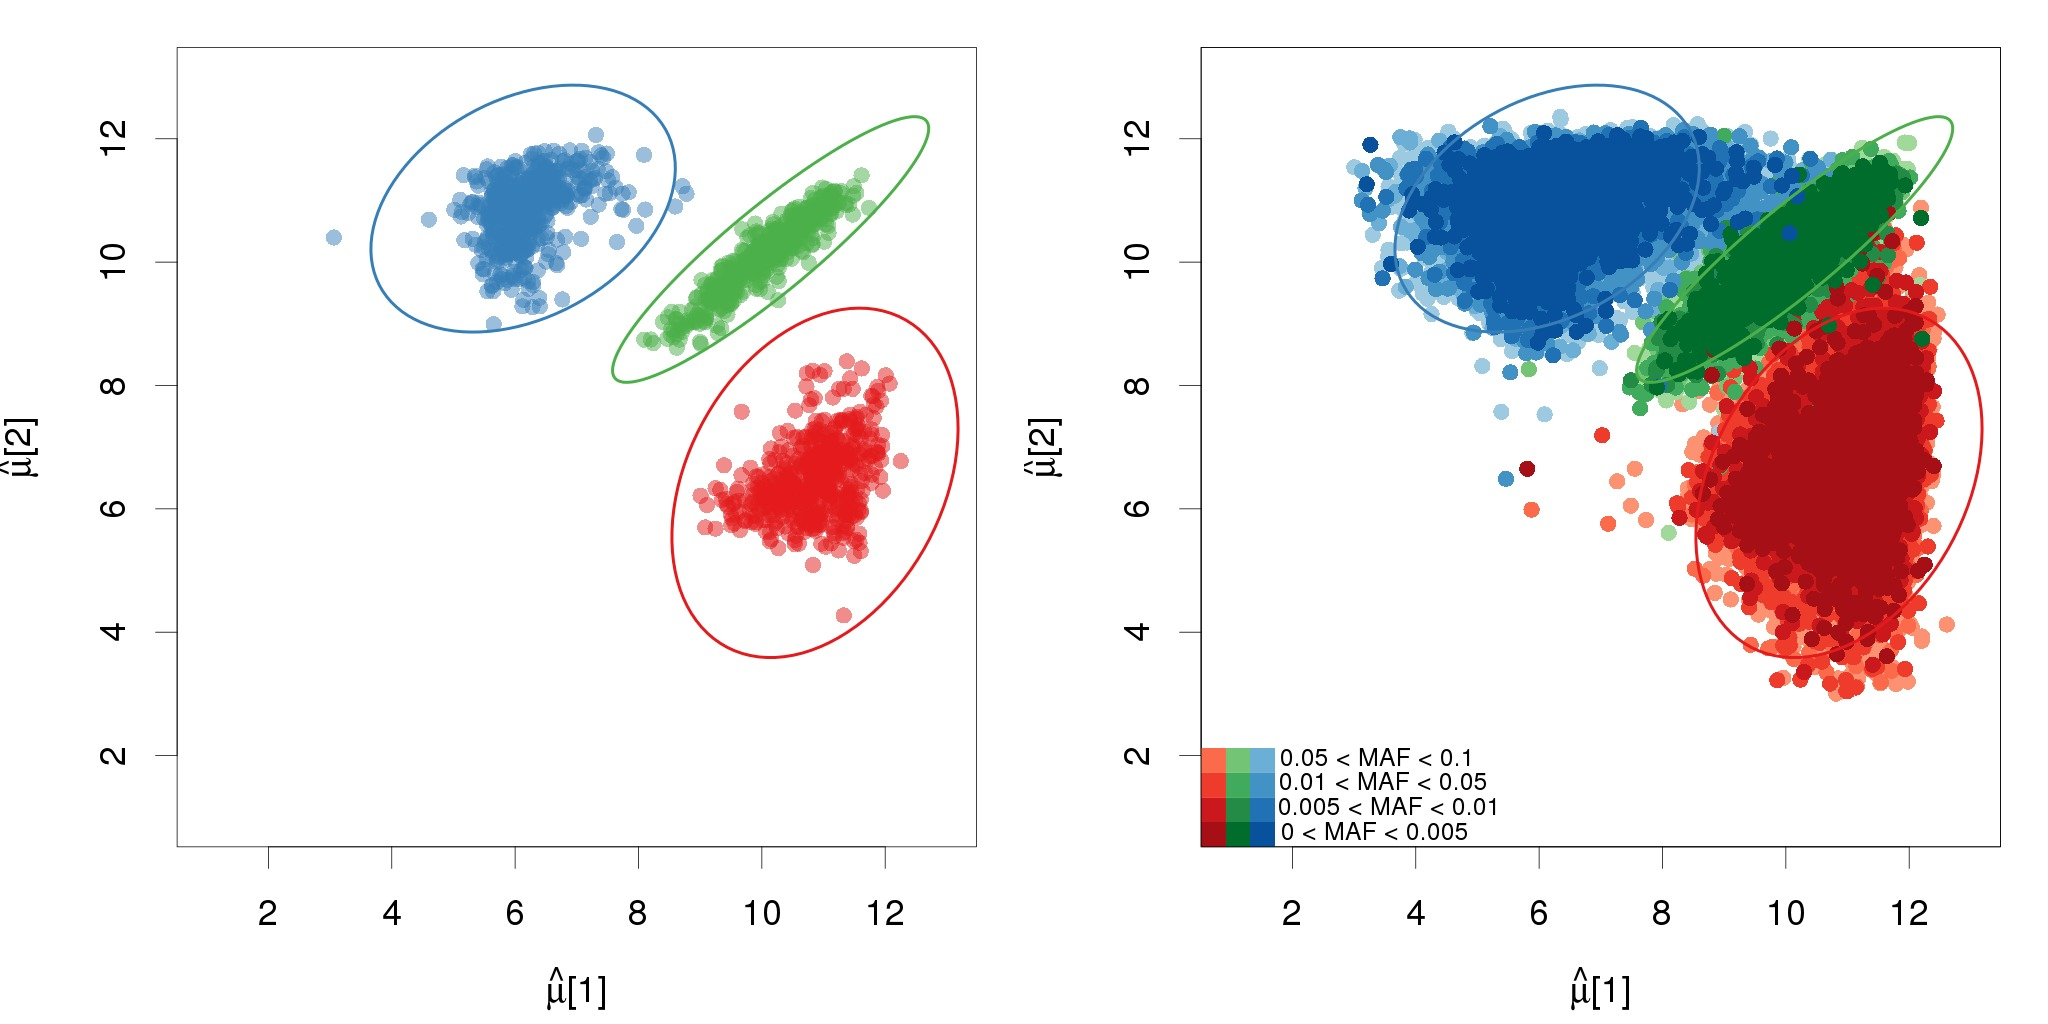
\includegraphics[width=\textwidth]{chap2figs/SupFig5}\\
    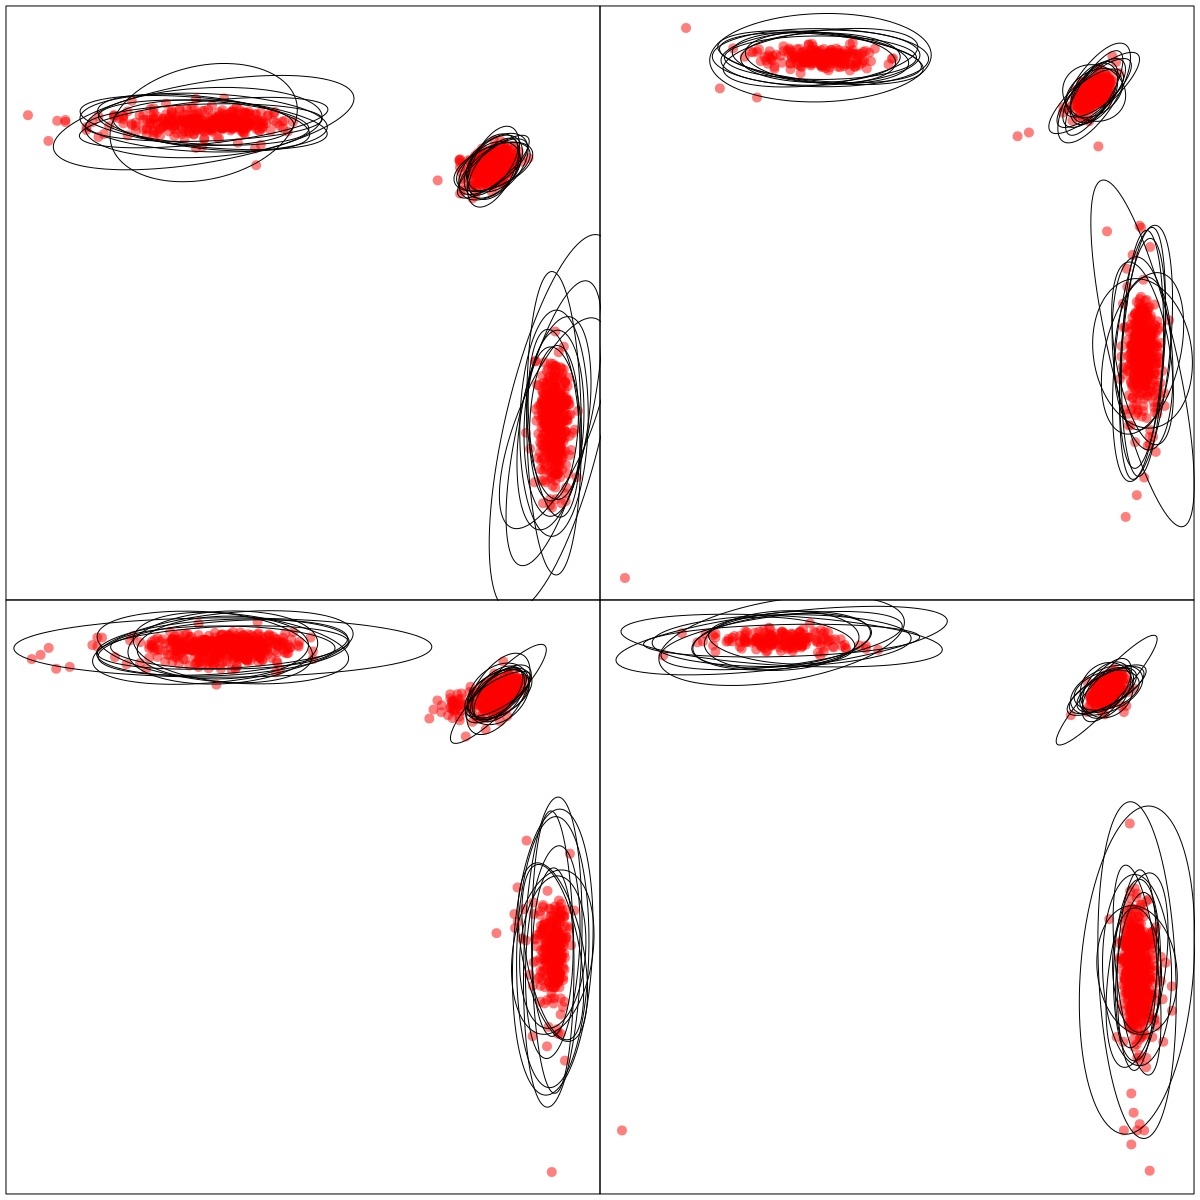
\includegraphics[width=.8\textwidth]{chap2figs/SupFig6}
    \caption[Comparison of priors and MAP estimates for our genotype calling model]{\textbf{Top left:} The estimated centroids for 1000 SNPs, the contour is the 99.9\% confidence interval of the centroid prior. \textbf{Top right:} MAP estimates of centroids (using array and sequence data) for 55126 SNPs on chromosome 20 with points shaded according to MAF.  There does not appear to be any strong relation between allele frequency and centroid location. \textbf{Bottom:} Signal intensities from four SNPs with 99.9\% confidence contours of ten simulated covariance matrices from the prior.\label{priors1}}
  \end{center} 
\end{figure}

\begin{figure}
\begin{center} 
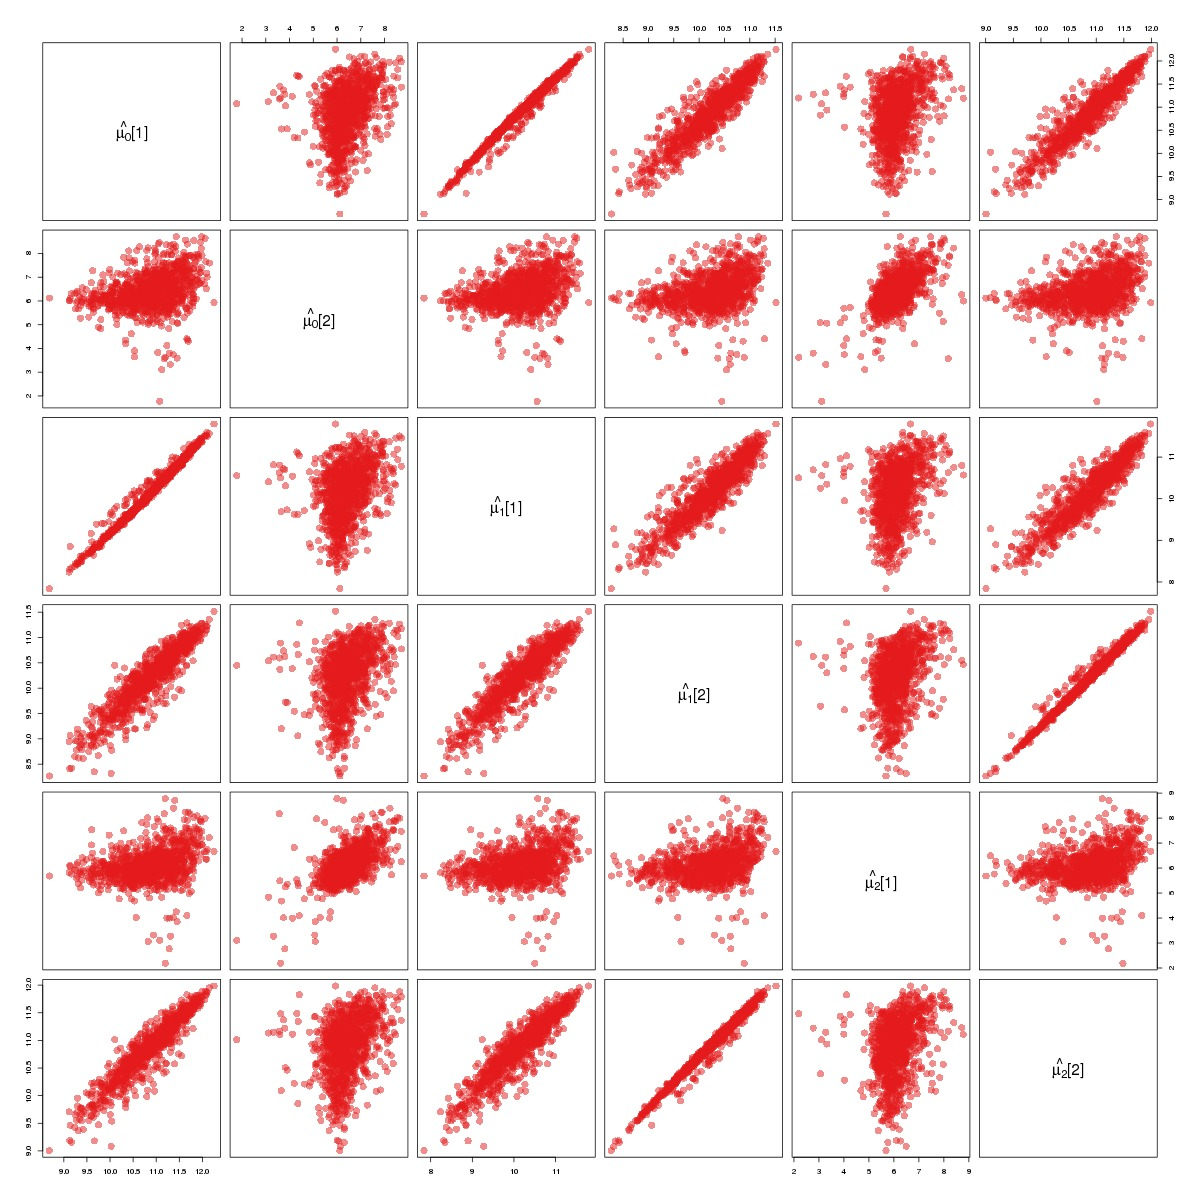
\includegraphics[width=\textwidth]{chap2figs/SupFig7}
\caption[Correlations between cluster centroids]{A pairs plot of the values for each mean estimate from the 1000 training SNPs.  We can see there is a strong correlation between the locations of the cluster centroids which may be exploited when choosing our priors.  The covariance of this data was used for the second (one off diagonal) and third priors.\label{mupairs}}
\end{center} 
\end{figure}
\clearpage
\subsubsection{Starting values}
Sensible starting values are crucial for fast convergence of our algorithm as well as converging to the desired mode of the posterior distribution.  Whilst the majority of SNPs have very good separation between genotype clusters, the location of the centroids of these clusters vary greatly between SNPs. Figure~\ref{centroid_eg} gives an example of two loci with high quality data but very different centroid locations. This means that using a constant set of starting values for parameters can be problematic. We undertook exploratory analyses on the centroid means estimated from easy SNPs to see if sensible starting values could be found from some simple sample statistic (for example, maximum allelic signal intensity).

We regressed each of the values in the three bivariate centroid means against the 95\% quantile of the allele intensity magnitude $\left( \sqrt{(X^1)^2+(X^2)^2} \right)$ for each allele, giving us six regressions in total.  We can see there is a strong relationship between  magnitude quantile and the centroids of the clusters (Figures~\ref{reg1}).  We exploit this relationship to select starting values that allow quick convergence of our ECM algorithm to the desired mode by calculating the quantile at each SNP and setting the centroid starting values according to the least squares estimates show in Figure~\ref{reg1}.

\begin{SCfigure}[1][h]
\centering
    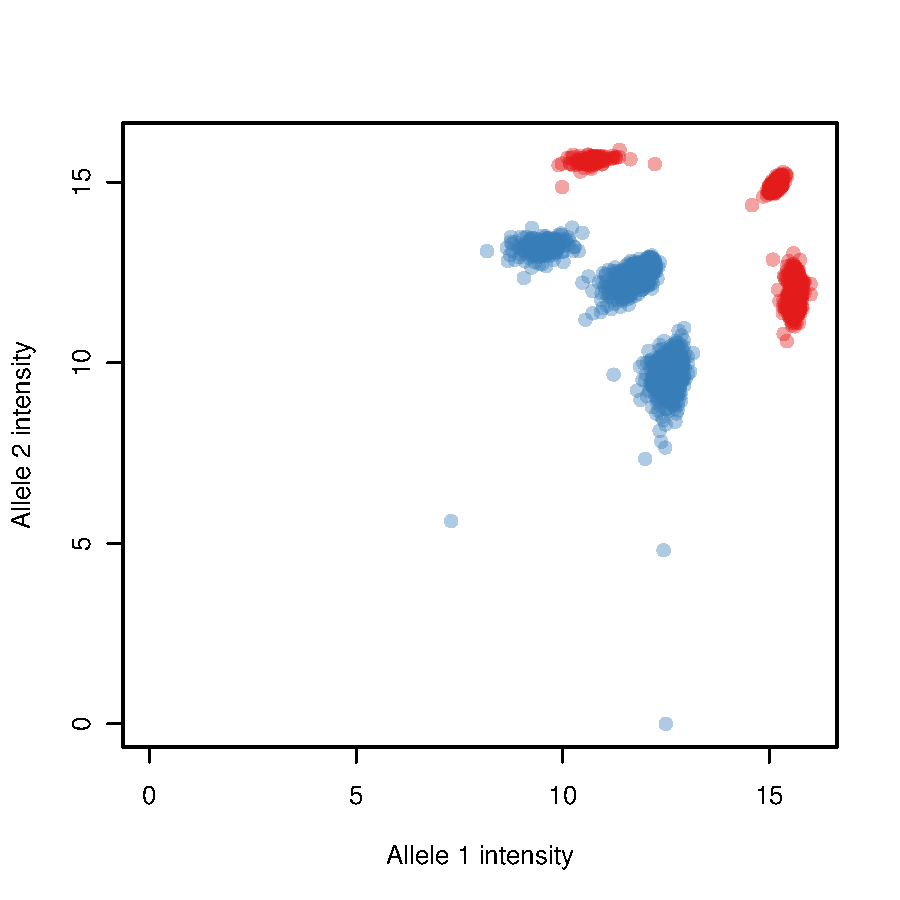
\includegraphics[width=.5\textwidth]{chap2figs/SupFig1}
    \caption[Signal intensities from two SNPs with very different cluster locations]{Signal intensities from two separate SNPs, whilst discrimination is good, the locations of the cluster centroids vary greatly.  This makes it difficult to rely on constant starting values between SNPs.  \label{centroid_eg}}
\end{SCfigure}
\clearpage

\begin{figure}
 \begin{center}  
               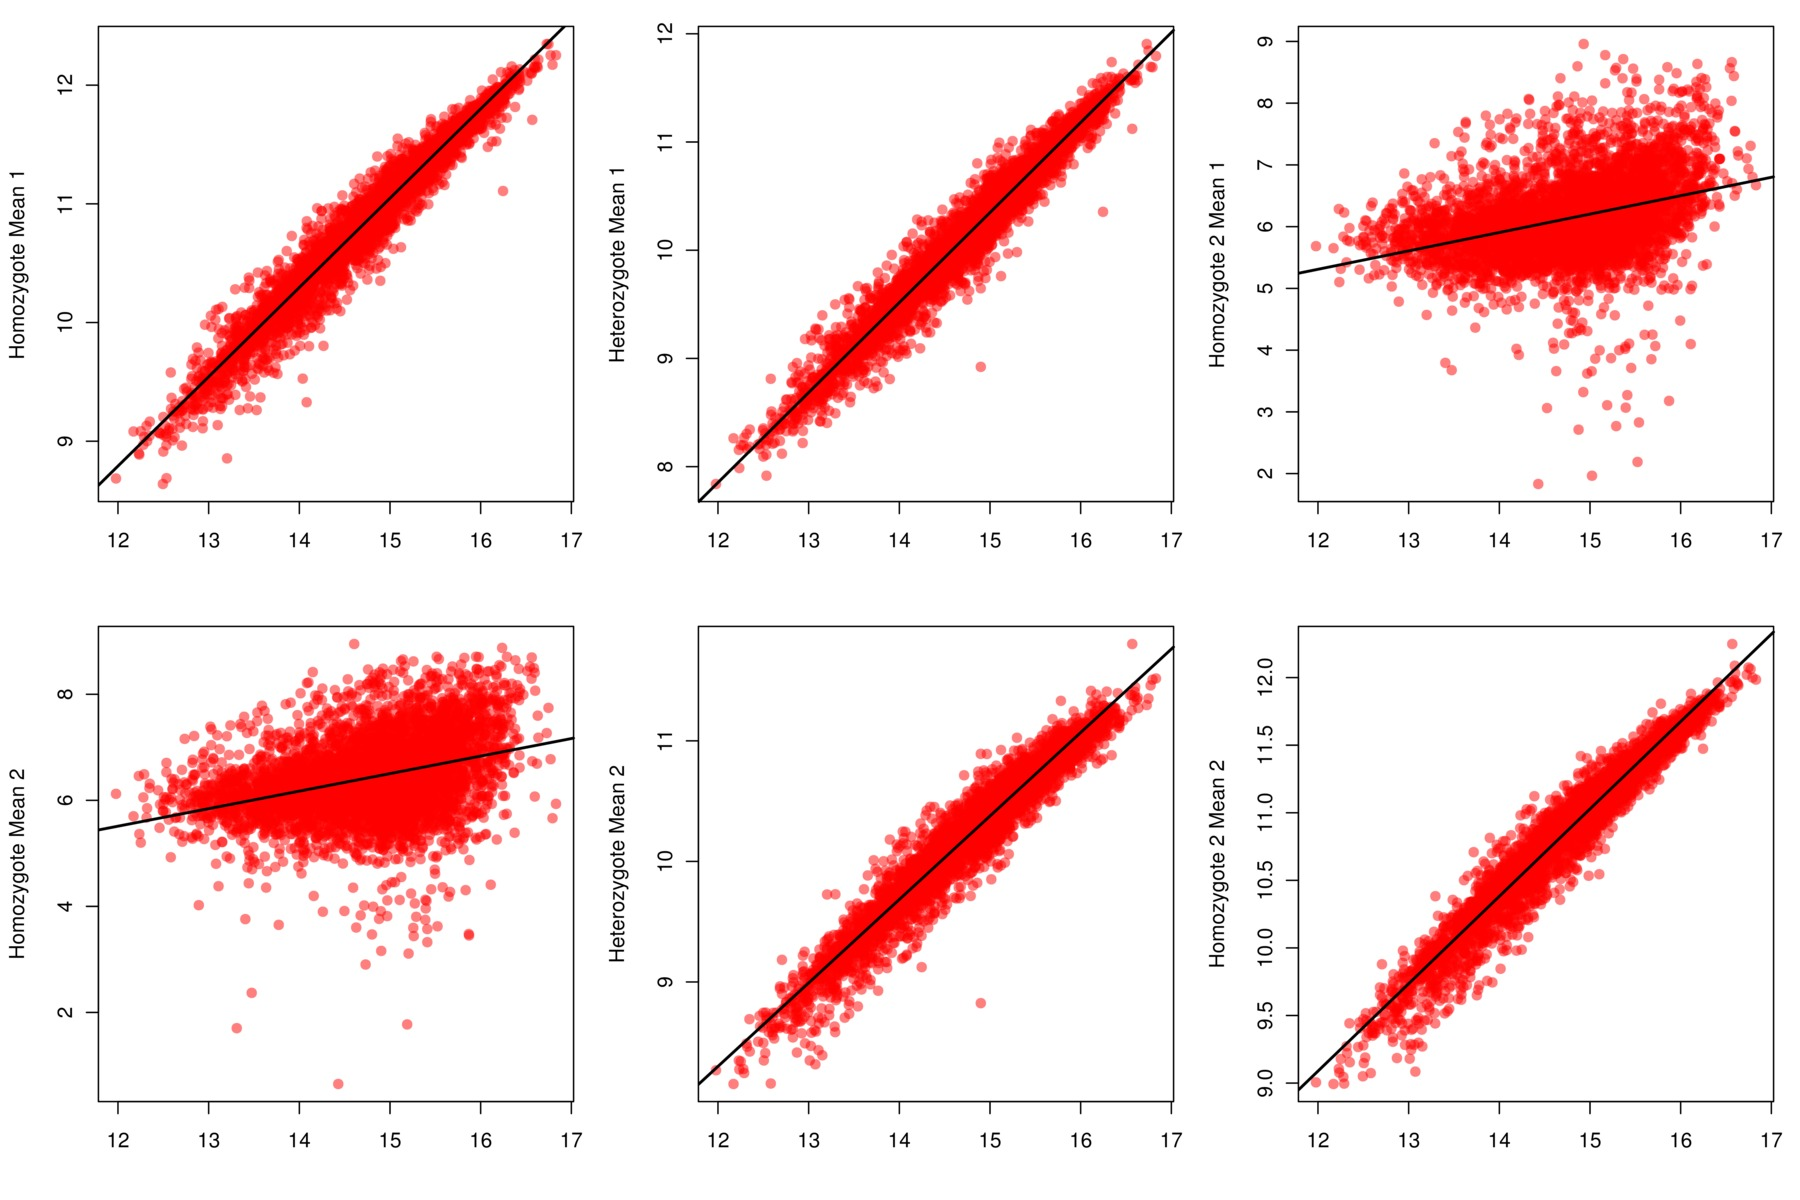
\includegraphics[width=\textwidth]{chap2figs/SupFig8}
\caption[Comparison between cluster centroids and maximum allele intensities]{The scalar elements of each centroid regressed against the 95\% quantile of the allele intensity magnitude. There is a strong relationship between this value and the location of the means.\label{reg1}}
\end{center} 
\end{figure}
\clearpage
\subsection{Posterior probabilities in output}
The Illuminus and GenoSNP methods both output posterior probabilities $P(G=j|\textrm{Data})$ for genotypes $G \in (0,1,2,\textrm{NULL})$. Observations are assigned to the ``NULL'' class by these methods when the array data does not appear to come from one of the three genotype clusters.  Our method uses two latent variables to indicate failed sequence and array assays for each genotype which allows us to call genotypes when at most one of the assays fails. This means when the failure parameters are high, causing $P(\textrm{Data}|G=j)$ to be flat, the posterior probability will tend towards to population frequency of the genotypes since we have no explicit ``NULL'' class.  This is reasonable behaviour but means our method is not directly comparable to other callers.  This is issue is easily circumvented by calculating a slightly different probability.

We calculate the posterior probability of a ``NULL'' genotype as the posterior probability that both assays have failed
\begin{eqnarray*}
P(G_i = \textrm{NULL}|X_i,Y_i)  &=& P(Z_i^X=1 \cap Z_i^Y=1|X_i,Y_i).
\end{eqnarray*}
We call genotypes when at least one of the assays has succeeded using
\begin{eqnarray*}
 P(G_i = j|X_i,Y_i,Z_i^X=0 \cup Z_i^Y=0) &\propto& P(G=j) P(X_i,Y_i|Z_i^X=0 \cup Z_i^Y=0) \qquad j \in {0,1,2}.
\end{eqnarray*}

We use these probability values for methods evaluation in section~\ref{chap2:results:comparison} as it makes Illuminus, GenoSNP and Chiamante directly comparable. GenTrain2 does not provide a posterior probability per genotype although does flag genotypes as missing when the array data is atypical, we just take the hard calls from GenTrain2.


\section{Data sets}
\label{chap2:data}
We evaluated our method in several ways using real data from Phase 1 of the 1000 Genomes Project. The data consist of a total of 1,525 samples from 15 populations. There are 1,525 samples with allele intensity data from the Illumina Omni2.5S genotyping chip. A subset of 1094 of these samples also have low-coverage (4X) sequencing data available, summarised in the form of genotype likelihoods.   In addition, we used genotype data on 1261 samples from an Affymetrix Axiom genotyping chip to assess the performance of methods, by taking the Affymetrix genotypes to constitute the true genotypes. There are 828 samples typed on both Omni2.5S and Axiom chips. There are 623 samples with data from all three technologies. This data is summarised in Figure~\ref{venn} and full details of the samples are in supplementary table~\ref{chap2:sampleinfo}.

\begin{SCfigure}[1][h]
\centering
    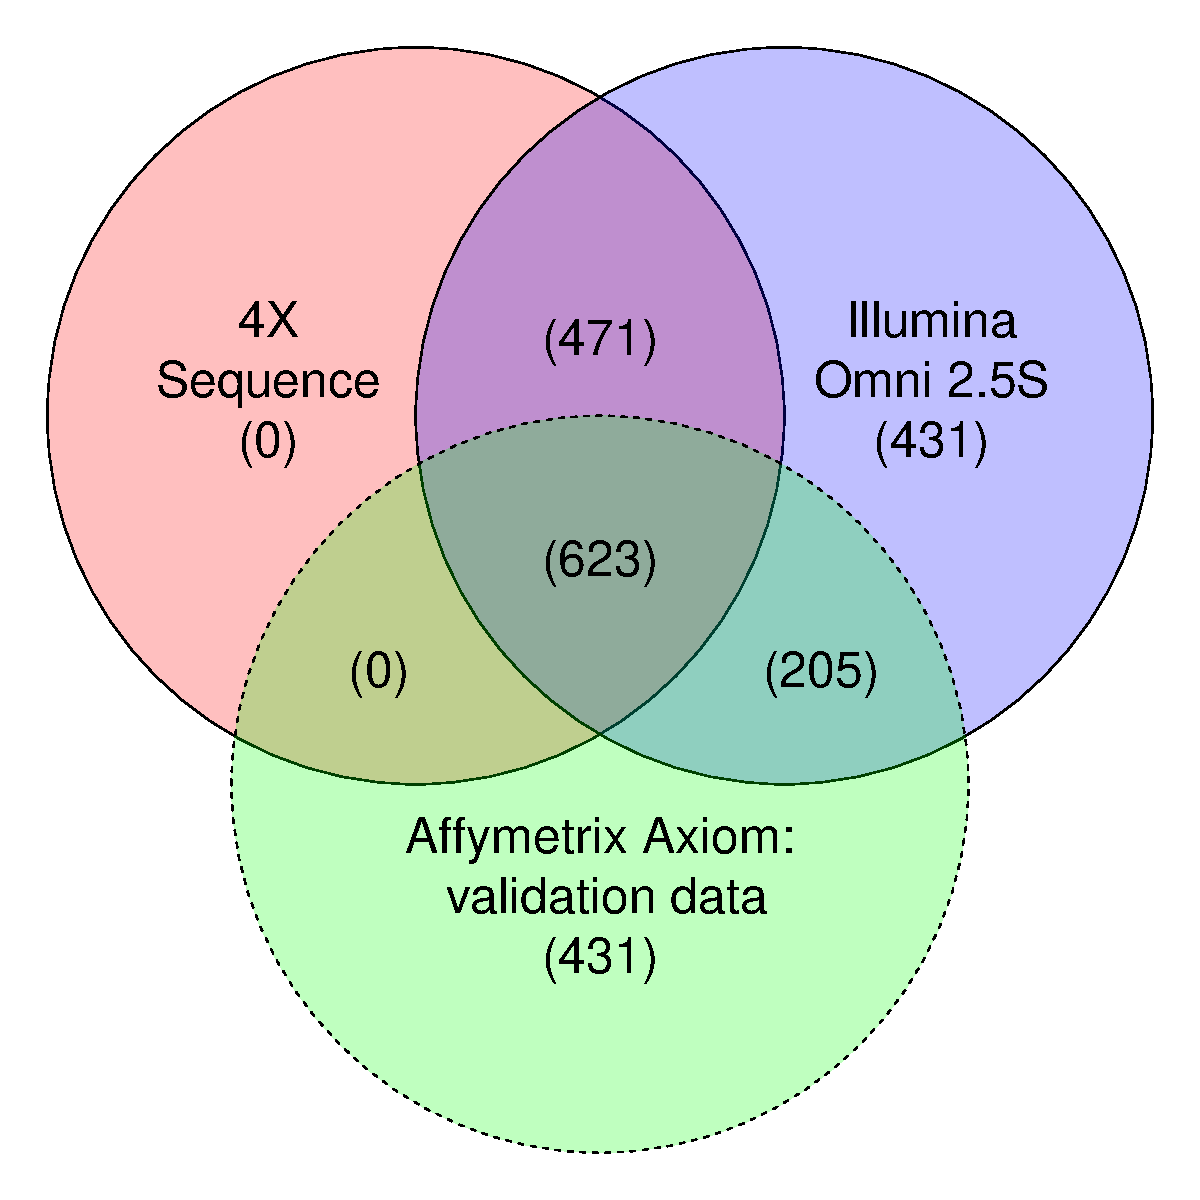
\includegraphics[width=.4\textwidth]{chap2figs/venn}
    \caption[The available samples assayed on each genotyping technology]{Venn diagram summarising the available samples assayed on each technology.  We developed models and made genotype calls for the sequence and Illumina Omni 2.5S data and used genotypes from the Affymetrix Axiom chip as validation data.  \label{venn} }
\end{SCfigure}


\subsection{Evaluating accuracy}
The easiest way to compare methods is to force each method to make a call of each genotype and then calculate the concordance with the calls made on the Axiom chip. In a real study it is usual to apply filters that exclude individual genotypes or whole SNPs that seem to have spurious genotype calls and then measure concordance on the genotypes that have passed the filters. We use the notation $\hat{G}_{il}$ to denote the genotype call made in the $i$th individual at the $l$th SNP. By default this genotype call (either 0, 1, 2 or NULL) will be the one which has the highest posterior probability. The result of applying a filter will be to set some of these genotype calls to NULL.

Once the filter has been applied we can calculate the genotype call rate (GCR), which is the percentage of all non-NULL genotypes, defined as 
\begin{equation}
\textrm{GCR} = 100 \times \frac{\sum_{i=1}^N \sum_{l=1}^L I(\hat{G}_{il}\neq \textrm{NULL})}{N \times L}
\end{equation}
and the percentage concordance of the non-NULL genotype calls with the non-NULL Affymetrix Axiom genotypes, defined as 

\begin{equation}
\textrm{Concordance} = 100 \times \frac{ \sum_{i=1}^N \sum_{j=0}^2 \sum_{l=1}^L I(G_{il}^{\textrm{Axiom}} = j) I(\hat{G}_{il}=j)}{\sum_{i=1}^N \sum_{l=1}^L I(G_{il}^{\textrm{Axiom}}\neq \textrm{NULL}) I(\hat{G}_{il}\neq \textrm{NULL}) } \label{concordance}
\end{equation}

We considered three standard filters. The first filter removes all genotypes with a posterior probability (PP) below 0.9. The second filter removes whole SNPs that show departures from Hardy-Weinberg Equilibrium (HWE). Since the data we use for the comparisons consists of multiple populations we calculate a p-value for a test of HWE in each of $M$ populations separately and then consider the minimum p-value across populations which has a Beta(1, $M$) distribution under the null of independent populations all in HWE. We exclude SNPs for which the resulting p-value is less that $10^{-7}$. The third filter removes whole SNPs where the SNP call rate (SCR) is below 0.9. SNP call rate is defined as the percentage of genotypes that were not NULL.  When the posterior probability filter is applied in conjunction with the SCR filter, a NULL genotype is defined as one having a posterior probability below 0.9. We consider all combinations of these filters which allows us to investigate the properties of our method compared to GenoSNP, Illuminus and GenTrain2. Note that GenTrain2 does not produce posterior probabilities so we just report the call rate and accuracy according to its hard genotype calls.


\clearpage
\section{Evaluating different genotype calling algorithms}
\label{chap2:results:comparison}

\subsection{Data sets with only array data on all samples} 

We compared our method to a range of other approaches  in the standard genotype calling scenario where only array data is available on the study samples. We called genotypes for the 1,525 1000 Genomes project individuals using only the Omni2.5S signal intensities (no sequence data) and assessed performance using the 828 individuals who were also assayed on the Affymetrix Axiom chip.  Table~\ref{chap2:arrayconc} shows the results of our method compared to Illuminus, GenoSNP and GenCall on the unfiltered data as well as all combinations of these filters. The table shows the overall call genotype call rate (GCR), the SNP call rate (SCR) and the concordance (Conc) for each method. Without any filters applied all the methods seem perform broadly the same with genotype call rates roughly between 99.72\% and 99.93\% and concordance between 99.63\% and 99.71\%. A more realistic comparison is how the methods perform after applying different QC filters.

The different filters have different effects on the different methods. Possibly the most striking result is the filter on HWE which removes a relatively large number of SNPs for GenoSNP and Illuminus (but not Chiamante or GenTrain2). This filter removes 0.33\% and 0.5\% of SNPs for GenoSNP and Illuminus respectively without very much effect on concordance. Figure~\ref{seq1,525qq} highlights this feature of the methods further by showing the quantile-quantile plots of the HWE p-values for each method. The figure shows that substantially more SNPs have extreme HWE p-values when using GenoSNP and Illuminus compared to using Chiamante or GenTrain2. In practice, this translates to $>5000$ extra SNPs that would pass QC and hence be available for downstream analyses when using Chiamante or GenTrain2 versus Illuminus or GenoSNP.

When all the filters are combined we find that all the methods have a Concordance of between 99.71\%-99.73\% but the methods have differing GCR and SCR. Chiamante increases GCR over GenoSNP and Illuminus by 1\% and 0.1\% respectively. It also increases SCR over GenoSNP and Illuminus by 0.9\% and 0.2\% respectively. Comparing all the methods when just the SCR and HWE filters are applied the best two methods are Chiamante and GenTrain2. The concordance between these two methods is roughly the same, Chiamante has a better GCR by 0.03\% and GenTrain2 has a better SCR by 0.07\%. 

We also examined the effect of each individual filter on the different methods by varying the filter thresholds. Figure~\ref{arrayfig} shows the percentage of missing data versus concordance for each of the methods as the filters thresholds are varied. This figure highlights how GenTrain2 seems remarkably robust to the various filters and that the PP and HWE filters have a much bigger effect on the performance of Illuminus and GenoSNP.  
%\begin{landscape}
\vspace{20pt}
\begin{table}[h]
\begin{center}
 \resizebox{\textwidth}{!}{
\begin{tabular}{|l|rrr|rrr|rrr|rrr|}
  \hline
  & \multicolumn{3}{c|}{Chiamante}& \multicolumn{3}{c|}{GenoSNP}& \multicolumn{3}{c|}{Illuminus} &\multicolumn{3}{c|}{GenTrain2}  \\
  \hline
 Filter & GCR & SCR & Conc & GCR & SCR & Conc& GCR & SCR & Conc& GCR & SCR & Conc\\
  \hline
  None & 99.824 & 100.000 & 99.696 & 99.802 & 100.000 & 99.632 & 99.930 & 100.000 & 99.670 & 99.720 & 100.000 & 99.707 \\ 
  \hline
  SCR & 99.646 & 99.765 & 99.698 & 99.516 & 99.634 & 99.666 & 99.877 & 99.927 & 99.678 & 99.605 & 99.822 & 99.710 \\ 
  HWE & 99.766 & 99.941 & 99.708 & 99.509 & 99.669 & 99.683 & 99.436 & 99.496 & 99.701 & 99.677 & 99.955 & 99.712 \\ 
  PP & 99.744 & 100.000 & 99.715 & 99.470 & 100.000 & 99.683 & 99.896 & 100.000 & 99.679 &  - & - & - \\
  \hline
  SCR+HWE & 99.590 & 99.710 & 99.709 & 99.345 & 99.457 & 99.693 & 99.406 & 99.455 & 99.706 & 99.568 & 99.783 & 99.714 \\ 
  PP+SCR & 99.520 & 99.694 & 99.722 & 98.605 & 98.857 & 99.710 & 99.826 & 99.905 & 99.692 &  - & - & - \\
  PP+HWE & 99.696 & 99.940 & 99.722 & 99.095 & 99.508 & 99.715 & 99.413 & 99.501 & 99.708 &  - & - & - \\
  \hline
  All & 99.486 & 99.659 & 99.726 & 98.508 & 98.756 & 99.721 & 99.381 & 99.456 & 99.713 & - & - & - \\
  \hline
\end{tabular}
}
 \caption[Genotype calling  performance and effect of different QC filters]{Genotype call rate (GCR), SNP call rate (SCR) and concordance (Conc) in \% for different genotype calling methods applied to 1,525 samples assayed on the Omni2.5S chip and validated against a subset of 828 of these samples also assayed on the Affymetrix platform. Each row corresponds to a different combination of filters applied to the data. The PP filter removes all genotypes with a posterior probability below 0.9.  The HWE filter removes whole SNPs that show departures from HWE. The SCR  filter removes whole SNPs where the call rate is below 0.9. Call rate is defined at the percentage of genotypes that were not ``NULL'' }
\label{chap2:arrayconc}
\end{center}
\end{table}
%\end{landscape}

\begin{SCfigure}
\centering
    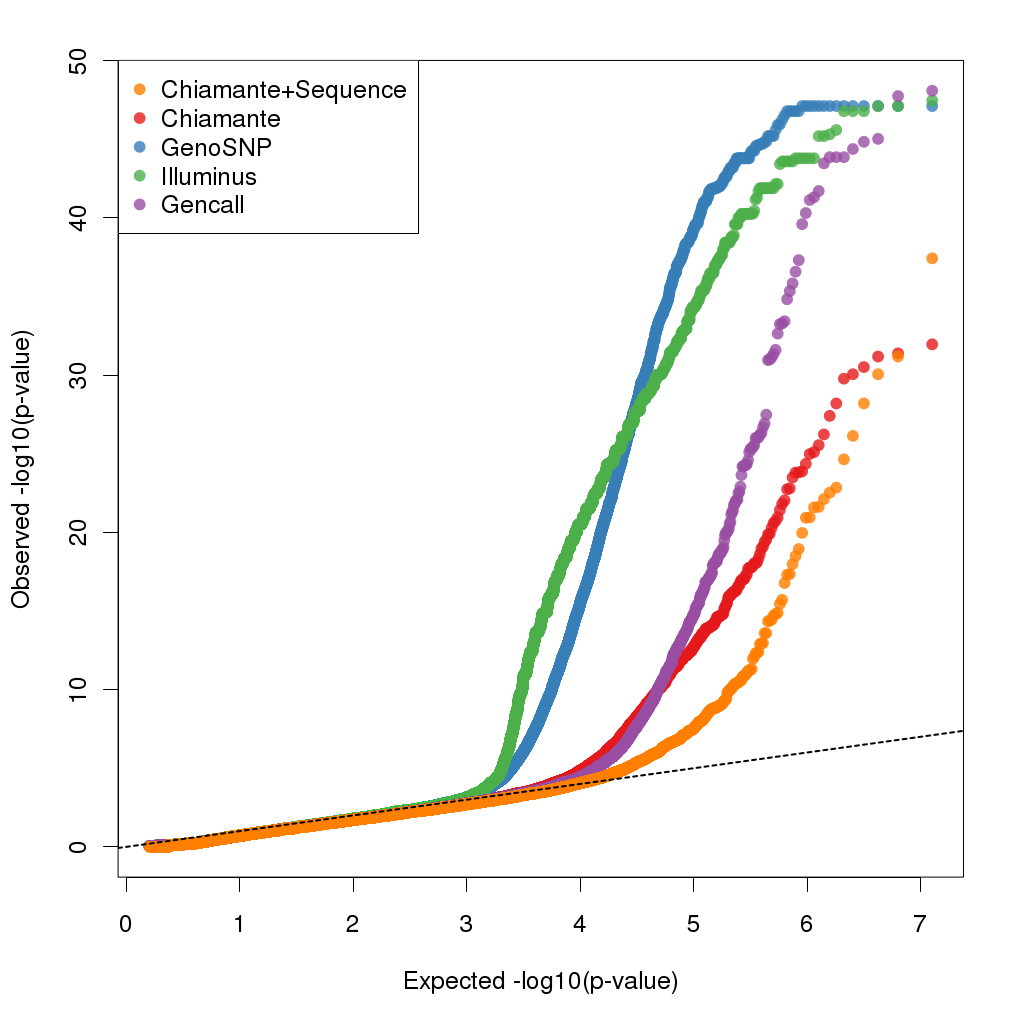
\includegraphics[width=.5\textwidth]{chap2figs/Fig3}
    \caption[Q-Q plots of HWE p-values for different genotype calling methods]{Q-Q plots of observed versus expected HWE p-values for different methods. Calls were made using each algorithm applied to Omni2.5S data from 1,525 individuals (17 different populations). The p-value is calculated at each locus by considering the minimum of the p-value for a test of HWE in each of $17$ populations separately which has a Beta(1, 17) distribution under the null of independent populations all in HWE.
      \label{seq1,525qq}}
\end{SCfigure}

\begin{figure}
  \begin{center} 
    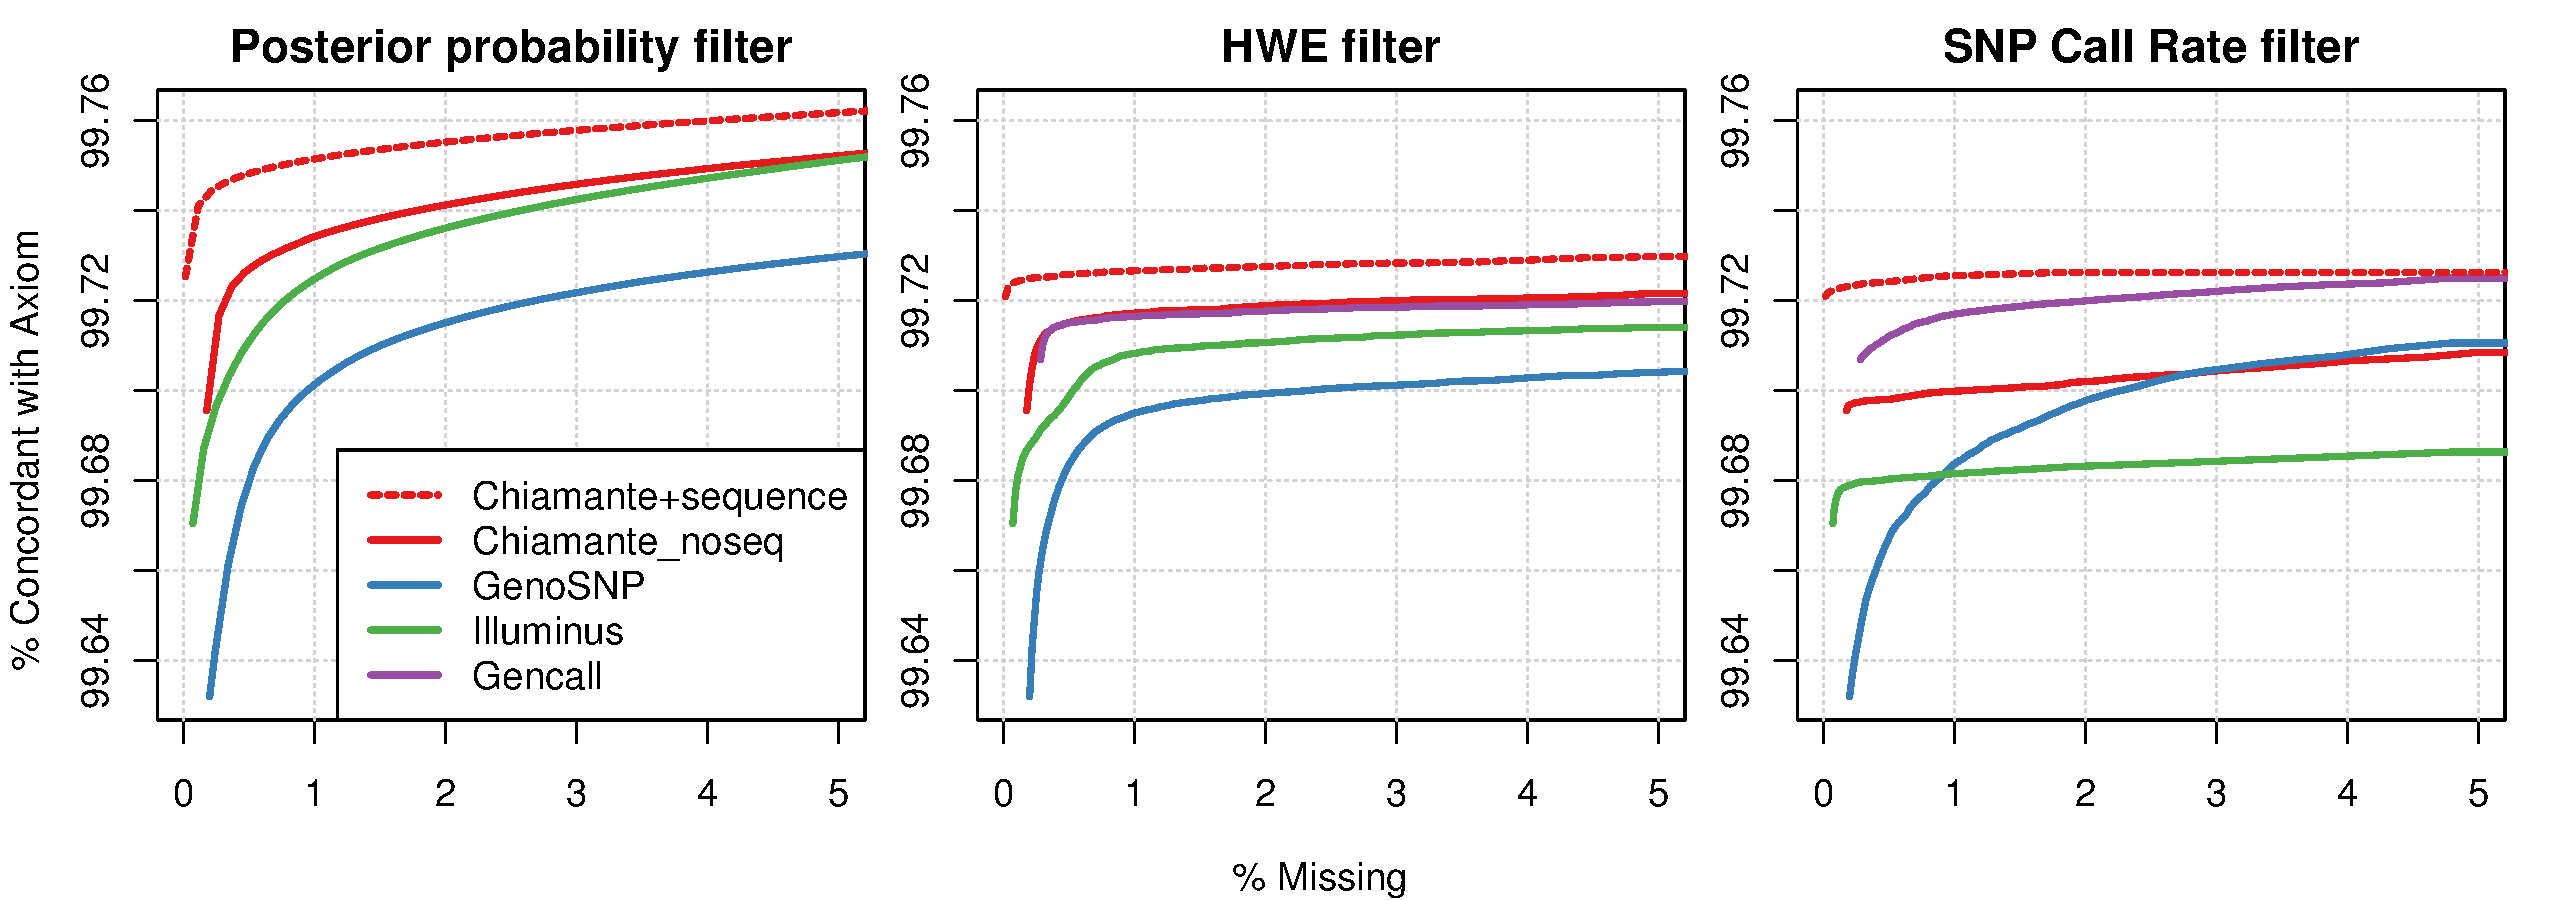
\includegraphics[width=\textwidth]{chap2figs/Fig2}
    \caption[Concordance against missingness for increasingly stringent QC filters]{Concordance against percentage missing data plots as increasingly stringent filter thresholds are applied. The left hand plot shows the effect of the filter on posterior probability (PP) of the methods Chiamante without using sequence data (red solid), Chiamante with use of sequence data (red dashed), GenoSNP (blue) and Illuminus (green). There is no comparison with GenTrain2 as the PP filter cannot be applied to this method. The middle plot show the effect of changing the threshold of the filter on HWE p-value. The right hand plot shows the effect of changing the threshold on the SNP call rate.\label{arrayfig}}
  \end{center} 
\end{figure}

\clearpage

\subsection{Data sets with a subset of samples with only array data and a subset of samples with both sequencing and array data} 

Having established that our method performs well in the situation in where only array data is available we investigated the gains in accuracy that could be achieved by utilising sequencing data on a subset of the samples. We again used the 1,525 individuals assayed on the Omni2.5S, 1,094 of these samples also have sequence data available. We applied our method with and without use of the sequence data. 

Table~\ref{tab_seq1,525}  shows the results of our method with and without the use of sequence data on the unfiltered data as well as all combinations of these filters. We examine performance on all 828 samples with Affymetrix Axiom data so that we can make a direct comparison with the results in Table~\ref{chap2:arrayconc} and shows clearly that overall the addition of sequence data leads to a clear boost in performance across a range of filtering options. When all the filters were applied the SCR, GCR and Concordance increase from 99.66, 99.487 and 99.727 to 99.954, 99.903 and 99.736. When sequence data is used the various filters have much less effect. For example, the GCR, SCR and Concordance never drop below 99.9\%, 99.95\% and 99.721\% respectively for any combination of filters. The fact that concordance does not seem to increase much (99.721\% without sequence data and 99.736\% with sequence data) maybe due to errors in the Axiom data that effectively put an upper bound on this measure that is below 100\%. 

\begin{table}[p]
\begin{center}
\begin{tabular}{|l|rrr|rrr|}
  \hline
  Method & \multicolumn{3}{c|}{Chiamante}& \multicolumn{3}{c|}{Chiamante+Sequence}\\
  \hline
  Filter & GCR & SCR & Conc & GCR & SCR & Conc \\ 
  \hline
  None & 99.824 & 100.000 & 99.696 & 99.986 & 100.000 & 99.721 \\ 
  GCR & 99.646 & 99.765 & 99.698 & 99.974 & 99.985 & 99.722 \\ 
  HWE & 99.766 & 99.941 & 99.708 & 99.970 & 99.984 & 99.723 \\ 
  PP & 99.744 & 100.000 & 99.715 & 99.940 & 100.000 & 99.733 \\ 
  \hline
  GCR+HWE & 99.590 & 99.710 & 99.709 & 99.958 & 99.969 & 99.723 \\ 
  PP+GCR & 99.520 & 99.694 & 99.722 & 99.914 & 99.966 & 99.734 \\ 
  PP+HWE & 99.696 & 99.940 & 99.722 & 99.927 & 99.986 & 99.734 \\ 
  \hline
  All & 99.486 & 99.659 & 99.726 & 99.903 & 99.954 & 99.736 \\ 
  \hline
\end{tabular}
\caption[Performance with and without and with the use of sequence data. ]{Comparison of Chiamante's performance applied to the 1,525 samples with data from the Illumina Omni2.5S chip without (left) and with (right) the use of sequence data. Genotype call rate (GCR), SNP call rate (SCR) and concordance (Conc) with the Affymetrix Axiom chip in \% are listed for each call set. Table rows correspond to a different combination of filters applied to the data. The PP filter removes all genotypes with a posterior probability below 0.9.  The HWE filter removes whole SNPs that show departures from HWE. The GCR filter removes whole SNPs where the call rate is below 0.9. Call rate is defined at the percentage of genotypes that were not ``NULL''.}
\label{tab_seq1,525}
\end{center}
\end{table}

\begin{figure}[p]
  \begin{center} 
    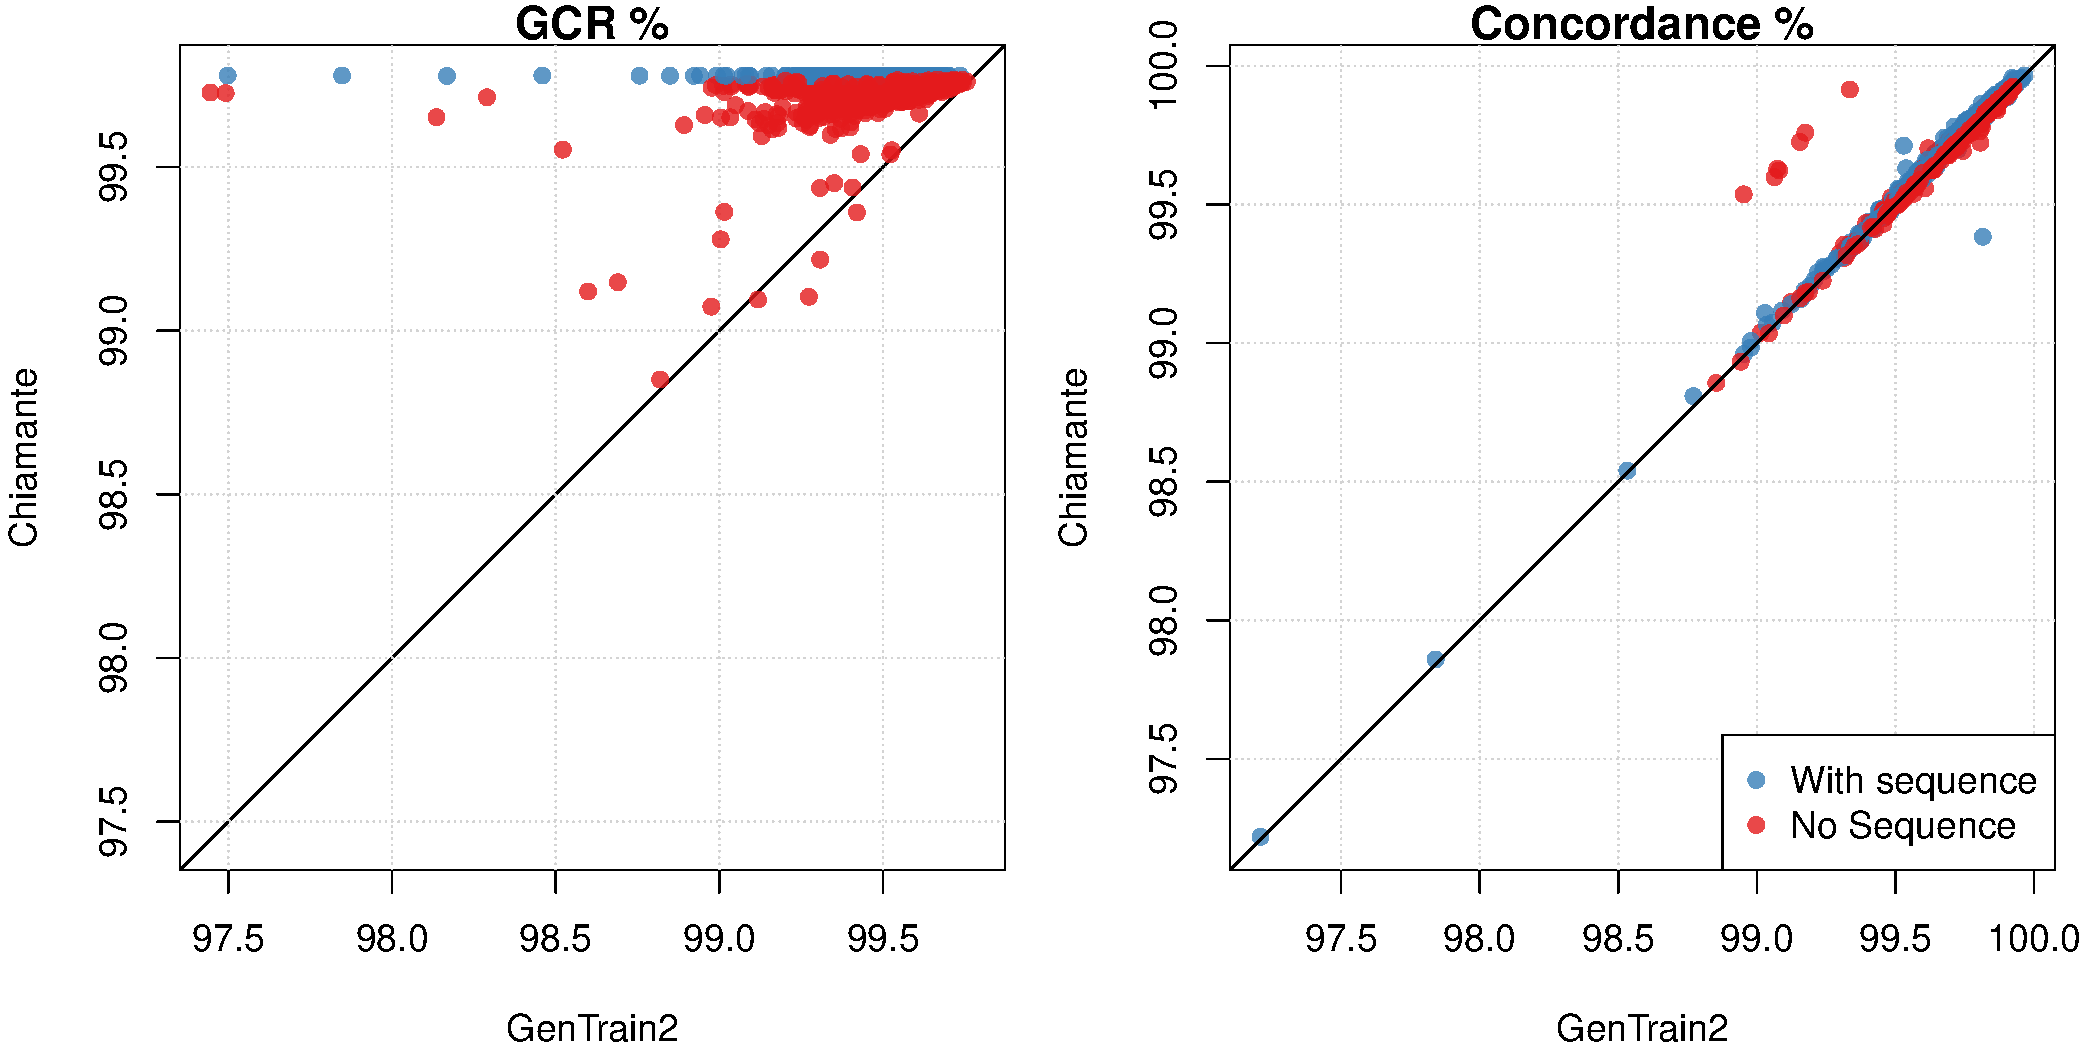
\includegraphics[width=\textwidth]{chap2figs/genotypecalling_byindv}
    \caption[Chiamante versus GenTrain2: per sample performance]{Chiamante+Sequence metrics versus GenTrain2 metrics for 828 individuals assayed on both microarrays.  The blue points are individuals that also have sequence data available, the red points are individuals whom were only assayed on microarrays. We can see that concordance is roughly the same between both methods but GCR is substantially larger for Chiamante+Sequence.  It is notable that there is improvement both for sequenced and non-sequenced samples.\label{seqnoseq}}
  \end{center} 
\end{figure}

Figure~\ref{arrayfig} shows the advantages of combining sequence and array data (red dotted line) compared to the methods that do not use sequence data via the missing data versus concordance plots. Figure~\ref{seq1,525qq} shows quantile-quantile plots for the HWE p-values for the different methods and further highlights that combining sequence and array data can noticeably reduce the number of SNPs failing HWE filters. Both highlight the ability of Chiamante+Sequence to improve call rate whilst maintaining accuracy.
\newpage
So far we have described metrics on 828 validation individuals, but 205 of these do not have any sequencing data available.  It is interesting to see if these individuals also have improved calls, or just the sequenced individuals. Figure~\ref{seqnoseq} plots metrics for Chiamante+Sequence versus GenTrain2 for each individual and colours points according to whether individuals are sequenced or not. There is improvement for individuals with no sequence data as well as the sequenced individuals,  we suspect this is due to the sequence data leading to improved model fit, hence benefiting all samples. In table~\ref{chap2:results:splitchi} we have split the results on the 828 samples with Axiom data into the subset of 623 that have 4X sequence data available and the remaining 205 samples that have no sequence data. The GCR and Concordance on the 205 samples are 99.423\% and 99.728\% when no sequence data is used and all post-calling filters have been applied. When sequence data is used on the calling the GCR rises by 0.4\% to 99.841\% and there is a slight rise in Concordance to 99.732\%.

Perhaps of greatest interest are the gains that can me made from using a combination of array and sequence at low frequency variants.  To evaluate this we took sites with a minor allele frequency less than 0.05 across all populations (estimated from the Axiom data) giving us 62,666 loci with 33,759,388 genotype calls (31,807,602 major homozygotes, 1,868,371 heterozygotes and 83,415 minor homozygotes). 

We then calculate sensitivity and specificity for each genotype $j$ and method, where
$$\textrm{Sensitivity}_j = 100 \times  \frac{\sum_{i=1}^N I(\hat{G}_{i=1} = j)I(G^{\textrm{Axiom}}_{i=1} = j)}{ \sum_{i=1}^N I(G^{\textrm{Axiom}}_{i=1} = j)} \qquad j \in (0,1,2,\textrm{NULL}))$$
$$\textrm{Specificity}_j = 100 \times  \frac{\sum_{i=1}^N I(G_{i=1} = j)I(G^{\textrm{Axiom}}_{i=1} = j \cap G^{\textrm{Axiom}}_{i=1} \neq \textrm{NULL})}{ \sum_{i=1}^N I(\hat{G}_{i=1} = j \cap G^{\textrm{Axiom}}_{i=1} \neq \textrm{NULL})}$$
that is, sensitivity is the percentage of the ``true genotypes'' (defined by Axiom) called by a method whilst specificity is the percentage of genotypes called by a method that are correct. 
\newpage
In this low frequency scenario we see more substantial improvements. The results are shown in Table \ref{1094tab4}. Chiamante (with sequence) has consistently higher detection rate and lower false discovery rate for all genotypes compared to the other methods.  In particular, we identify an extra 0.3\% minor homozygotes with 1.8\% fewer false positives compared to GenoSNP (the next best method for minor homozygotes).  We detect an additional 0.27\% heterozygotes with 0.25\% fewer false positives compared to GenCall, the next best method for heterozygotes. It is important to note here that the Axiom chip is also likely to be inaccurate for low frequency variants hence the error rate will be inflated, however this is still a reasonable way to compare each method on a relative scale. Illuminus has a much lower specificity 80.4\% on minor homozygotes than all the other methods which are all above 88.7\%.  
\begin{table}
\begin{center}
\begin{tabular}{|ll|c|c|}
  \hline
%  & &Sensitivity (\%)  & Specificity (\%)\\ 
% Method & Genotype (G) &  $100 \times P(Call = G | Axiom = G)$ & $100 \times P(Axiom = G | Call = G)$ \\
 Method & Genotype (G) &TPR (\%) & 1-FDR (\%)\\
 \hline
          & Major homozygote   & 99.78178 & 99.90596 \\
 Chiamante& Heterozygote     & 98.11328 & 98.65827 \\
          & Minor Homozygote   & 95.62908 & 88.78019 \\
 \hline
                   & Major homozygote    & 99.94782 & 99.90693 \\
 Chiamante+Sequence& Heterozygote     & 98.25222 & 99.19872 \\
                   & Minor Homozygote       & 96.11221 & 90.87426 \\
 \hline   
          & Major homozygote    & 99.78903 & 99.90625 \\
 GenoSNP & Heterozygote    & 97.95581 & 98.26359 \\
          & Minor Homozygote    & 95.81610 & 89.10256 \\
 \hline
          & Major homozygote    & 99.80620 & 99.90755 \\
 Illuminus& Heterozygote      & 97.38227 & 98.06591 \\
          & Minor Homozygote    & 95.28982 & 80.46608 \\
\hline
        & Major homozygote        & 99.67136 & 99.90829 \\
 GenCall& Heterozygote     & 97.98680 & 98.94823 \\ 
        & Minor Homozygote      & 95.60631 & 89.88650 \\
 \hline

\end{tabular}
\caption[Genotype calling performance at low frequency SNPs]{Sensitivity and specificity per genotype (for variants with MAF $<$ 0.05) for different calling methods using array data (and in Chiamante's case, sequence data) from 1094 individuals with validation data on a subset of 623 of these individuals.  Chiamante calls a higher rate of the low frequency variants whilst maintaining better sensitivity (true positive rate) and precision (1 - false discovery rate).}
\label{1094tab4}
\end{center}
\end{table}

\clearpage
To further illustrate the performance of our method and the benefit of using sequence and array data together Figure~\ref{chap2:fig:scatterplots} shows the cluster plots for three example SNPs shown on the three rows of the plot. The first column shows the cluster plots with points coloured using a RGB colour scheme based on the scaled GLs. In this way points that are very clearly coloured red, green and blue indicate genotypes where sequence data strongly supports reference homozygotes, heterozygotes and alternate homozygotes respectively. Genotypes for which the GLs are relatively flat across genotypes will be plotted as a mixture of red, green and blue. This way of plotting points helps to illustrate the general agreement between intensity clusters and GLs. The next three columns show the calls made by Chiamante, Illuminus and GenoSNP respectively. 

The first row shows an `easy' SNP where all methods agree. The second row shows a SNP where there are several points that lie between obvious clusters that could be hard to classify using array data alone. Here the use of sequence data leads to a boost in concordance by correctly classifying these ambiguous points. The third row shows a challenging SNP with atypical cluster centroids and where Allele 2 has low frequency, resulting in very few rare homozygotes which makes model fitting to array data only quite challenging. The concordance of Chiamante is considerably higher on this SNP due to both the use of sequence data and the priors we use on cluster locations which contribute to this increase in accuracy at rare SNPs.

\clearpage
\changepage{}{}{-.5in}{-.5in}{}{}{}{}{}
%\begin{landscape}
\begin{figure}
  \begin{center} 
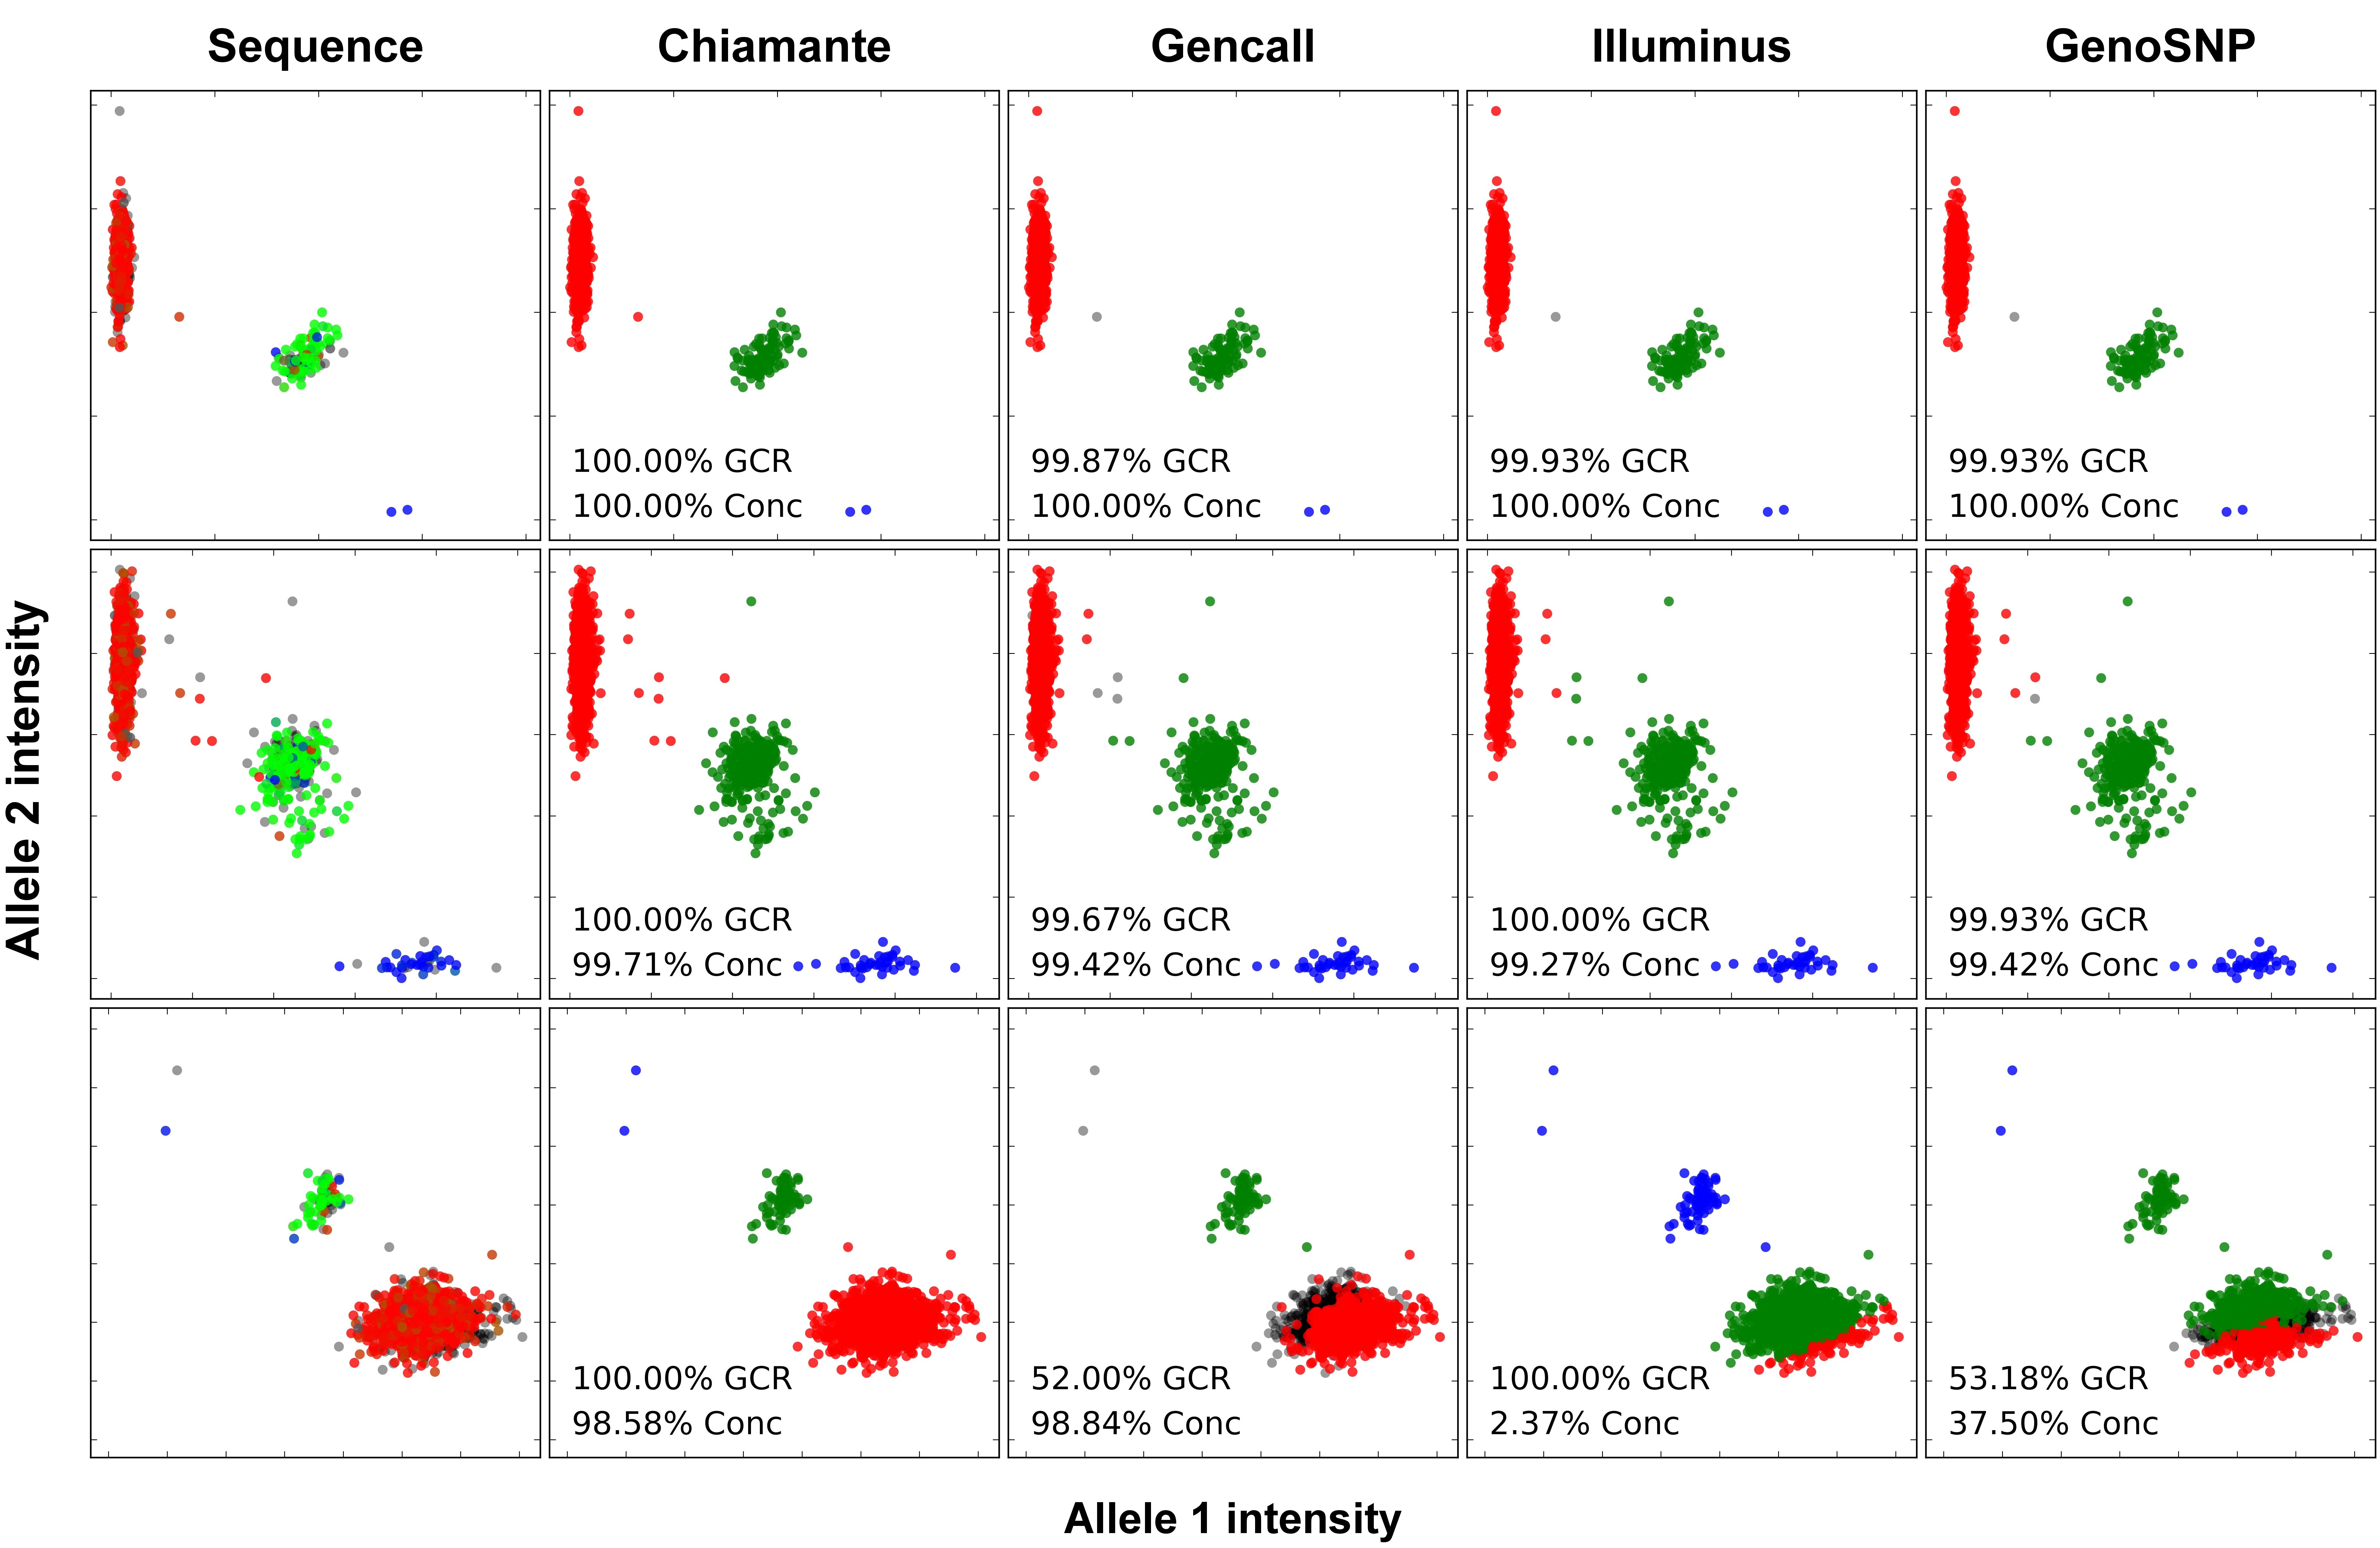
\includegraphics[width=\textwidth]{chap2figs/Fig4}
\vspace{-10pt}
    \caption[Scatter plots of allele intensities at three different loci of varying difficulty]{Scatter plots of allele intensities at three different loci.  In the far left column, points are coloured using a RGB colour scheme based on the scaled GLs. In this way points that are very clearly coloured red, green and blue indicate genotypes where sequence data strongly supports reference homozygotes, heterozygotes and alternate homozygotes respectively. Note the first probe of the Omni2.5S chip can be for either the reference or alternate allele so the colour of the homozygotes can differ between loci. Genotypes for which the GLs are relatively flat across genotypes will be plotted as grey.  The other four columns are coloured by genotypes from call sets generated by the respective algorithms. \textbf{Top:} Intensities from a typical well clustered SNP. The array-only methods call genotypes accurately but with one missed call.  Chiamante can `mop up' such ambiguous micro-array assays by exploiting the sequence information for this sample resulting in a higher call rate than the other callers. \textbf{Centre:} A more difficult SNP.   There are several uncertain samples between clusters which the other callers misclassify or exclude as missing, Chiamante can use the sequence information to accurately call these samples.  \textbf{Bottom:}  A SNP with relative low allele 2 frequency.  Illuminus and GenoSNP have both completely failed at this locus (this is likely due to incorrect convergence in the Illuminus case) whilst GenTrain2 has a large amount of missing data.  This SNP would typically be filtered in any reasonable QC pipeline.  The sequence data drives Chiamante to the correct parameter estimates for the mixture distribution resulting in accurate classification and high call rate at this locus.\label{chap2:fig:scatterplots}}
  \end{center} 
\end{figure}
%\end{landscape}
\changepage{}{}{+.5in}{+.5in}{}{}{}{}{}

\clearpage
\subsection{Examining errors}
\label{chap2:results:errors}
Our method estimates the rate at which the sequence and array assays have ``failed'' at each locus via the $\eta_Y$ and $\eta_X$ parameters respectively. Figure~\ref{chap2:results:eta_hist} shows histograms of these parameter estimates for all of the SNPs that were on the Illumina Omni2.5S chip and in the 1000 Genomes Phase I call set. The failure rate parameter for the sequence assay is noticeably elevated compared to the array assay. The majority of SNPs have an estimated sequence assay failure of between 0.001-0.0001, while  for the array assay the failure rates are almost always below 0.0001. 

We found that there were 754 SNPs with  $\eta_Y > 0.5$ but only 33 of these SNPs were on the Axiom array. Figure~\ref{chap2:results:eta_seq}  compares the properties of the calls at these SNPs with and without the use of sequence data. For the majority of the SNPs the calls are very similar with and without the use of sequence data, due to the sequence information being mostly discarded by the model.  There are some SNPs where the use of sequence data has led to greater divergence from HWE and some where the sequence data has modestly improved concordance. This suggests that model is largely robust to problematic sequencing data. Figure~\ref{seq_fail_1} shows a SNP flagged as having erroneous sequence level data ($\eta_Y = 0.63$). There is clear signal from the array assay showing good cluster separation whilst the sequencing data appears heavily biased towards the reference.  The model has correctly discarded the sequence data for many individuals at this locus and made high quality genotype calls (100\% Axiom concordance and call rate).

Figure~\ref{chap2:results:eta_array} shows various metrics for 235 SNPs that have the array failure rate,  $\eta_X > 0.5$ for Chiamante with and without sequence. The introduction of sequence data improves metrics on average, the HWE p-values are less extreme and both GCR and concordance are higher.  However call rates and concordance are frequently too low for these loci to be useful. Figure~\ref{array_fail_1} shows a typical example SNP flagged as having erroneous array level data ($\eta_X = 0.71$). There are a large number of points with 0 intensity, for most values here the genotype will be derived purely from sequence data.  The high concordance (98.6\%) should be considered in light of the very low call rate (73.9\%).  Such a locus is unlikely to be useful regardless of the calling method and would be filtered due to high missingness.

We have shown that our method is quite robust to extreme cases where the majority of sequencing or array data at a particular locus is spurious.  However these loci still tend to be of relatively poor quality and it may be to desirable to filter them.  Hence the two failure parameters may also be useful as quality control measures.  We calculated the average concordance for binned values of $-\log_{10}(\eta_X)$ and $-\log_{10}(\eta_Y)$ for Chiamante with and without sequence.   Figure \ref{fail_filtering} plots these averaged concordances against $-\log_{10}(\eta_X)$ and $-\log_{10}(\eta_Y)$.  The left panel shows how concordance changes with the array failure parameter, when sequencing data is present concordance is largely maintained even when array quality is low. However high values of $\eta_X$ will also lead to a large amount of missing values and SNPs are likely to be filtered on those grounds. The right plot shows concordance across the range of sequence failure rates, even when sequencing data is of poor quality Chiamante still benefits from its presence.  That said, low values of $\eta_Y$ tend to imply poor quality SNPs making this a useful QC parameter.  Filtering on $-\log_{10}(\eta_Y) <  2$ may be prudent and would result in the removal of only very few SNPs as can be seen in the histograms in Figure~\ref{chap2:results:eta_hist}.

\begin{figure}[p]
  \begin{center} 
    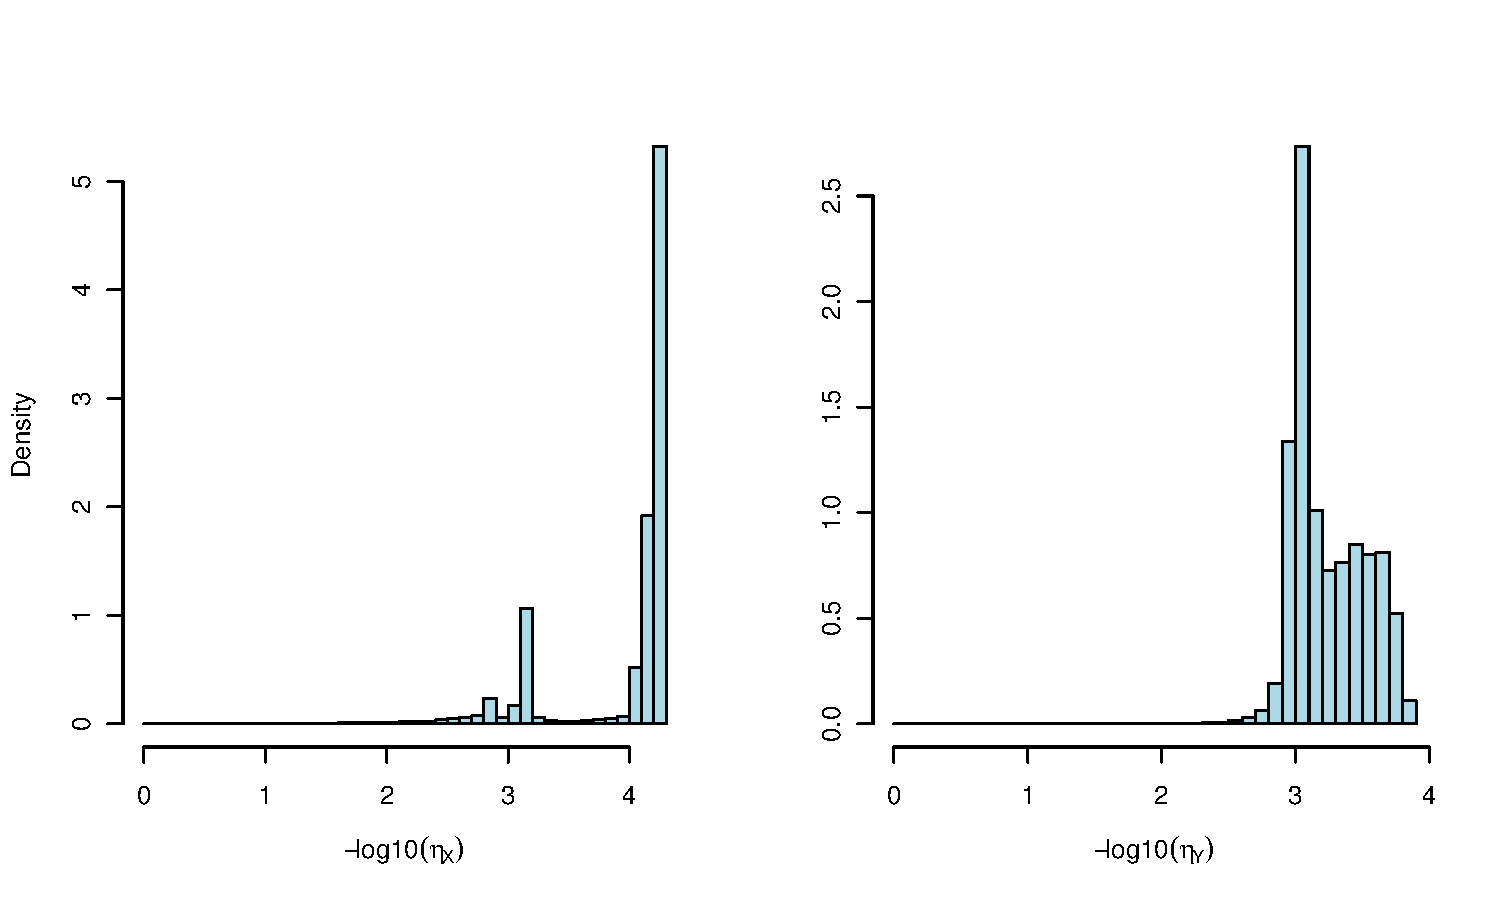
\includegraphics[width=\textwidth]{chap2figs/SupFig9}
    \caption[Histograms of the estimated failure rate parameters]{Histograms of the estimated failure rate parameters $-\log_{10} \eta_X$ for array assays (left) and $-\log_{10} \eta_Y$ for sequence assays (right).\label{chap2:results:eta_hist} }
  \end{center} 
\end{figure}


\begin{figure}[p]
  \begin{center} 
    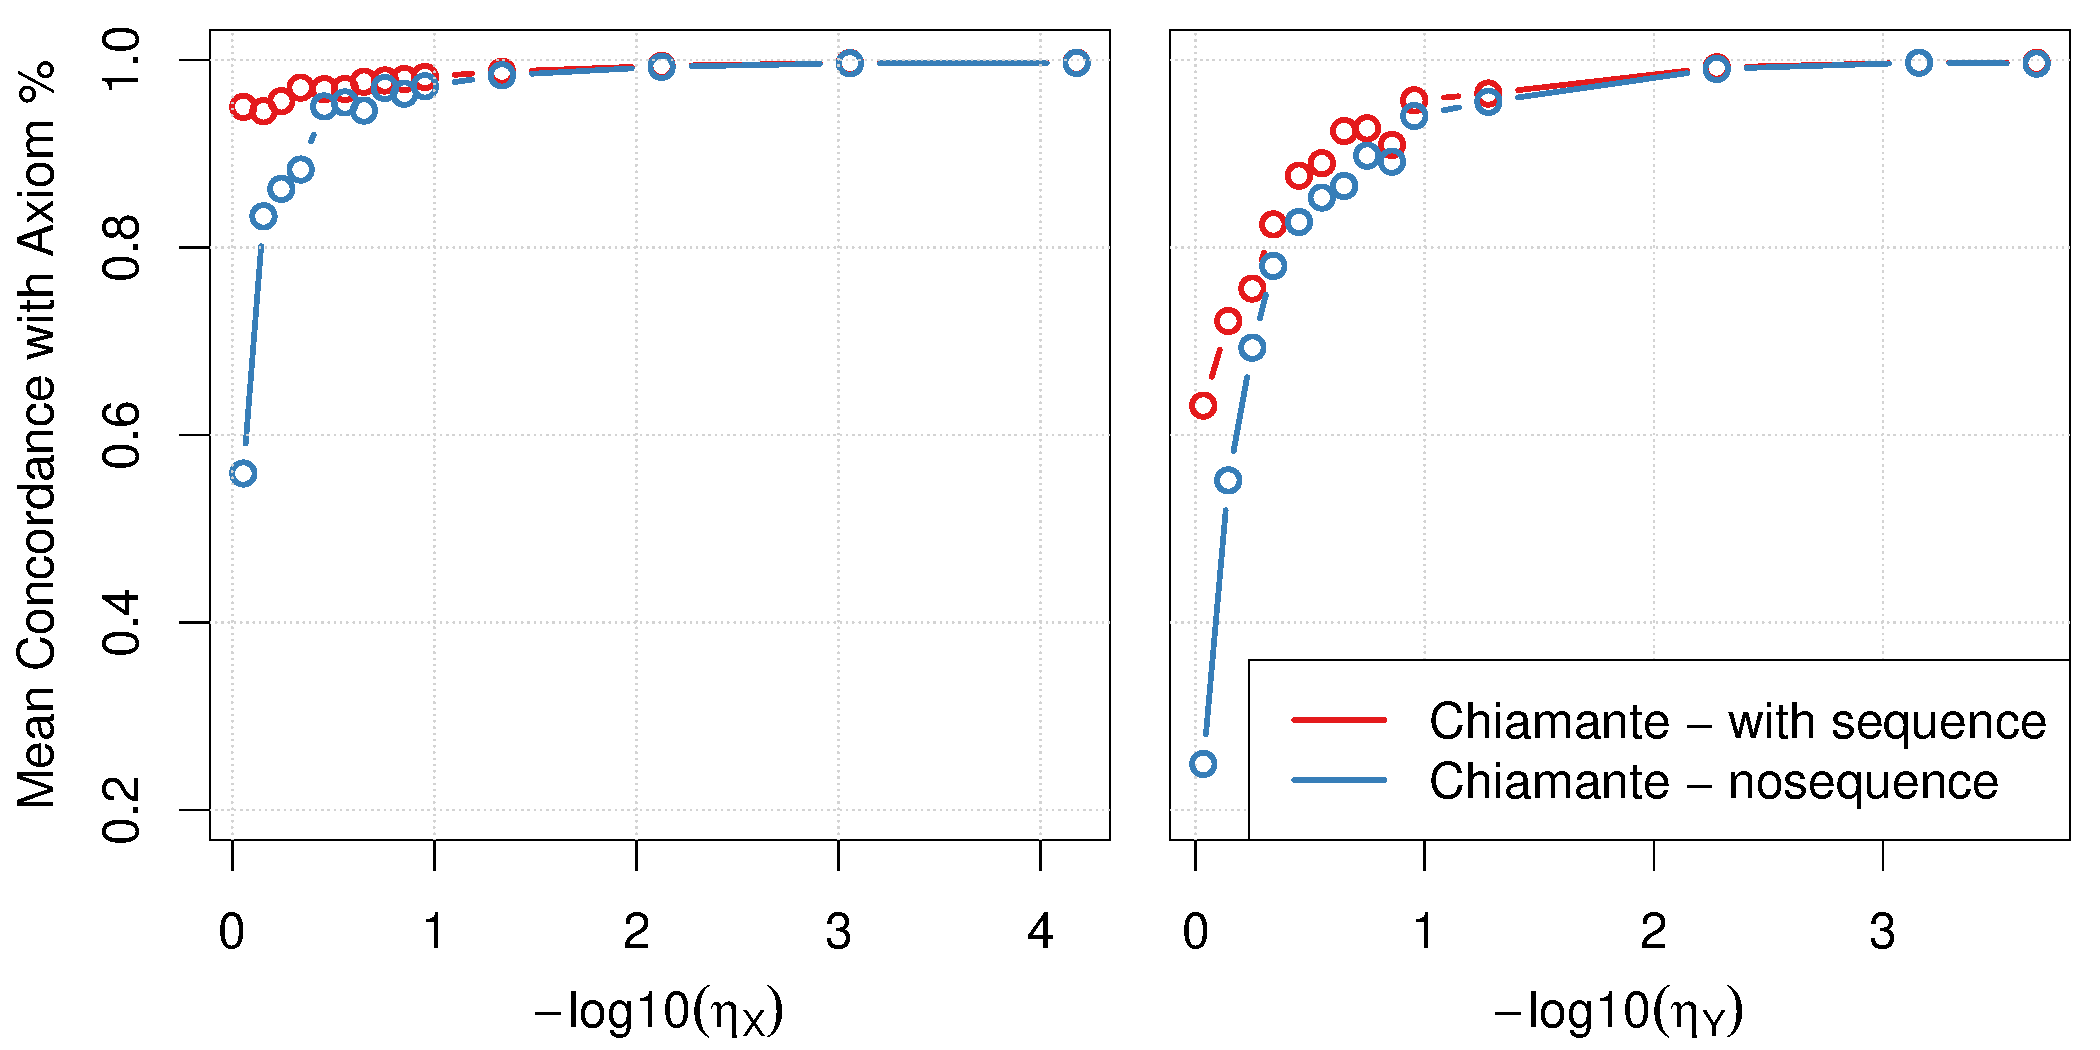
\includegraphics[width=\textwidth]{chap2figs/fail_filtering}
    \caption[Genotype concordance against rate of assay failure]{\textbf{Left:} Average concordance with Axiom against $-\log_{10} \eta_X$, the rate of array failure. \textbf{Right:} Average concordance with Axiom against $-\log_{10} \eta_Y$, the rate of sequence failure. Filtering SNPs with values of $-\log \eta_Y < 2$ may be a good additional QC measure.     \label{fail_filtering}}
  \end{center} 
\end{figure}

\begin{figure}[p]
  \begin{center} 
    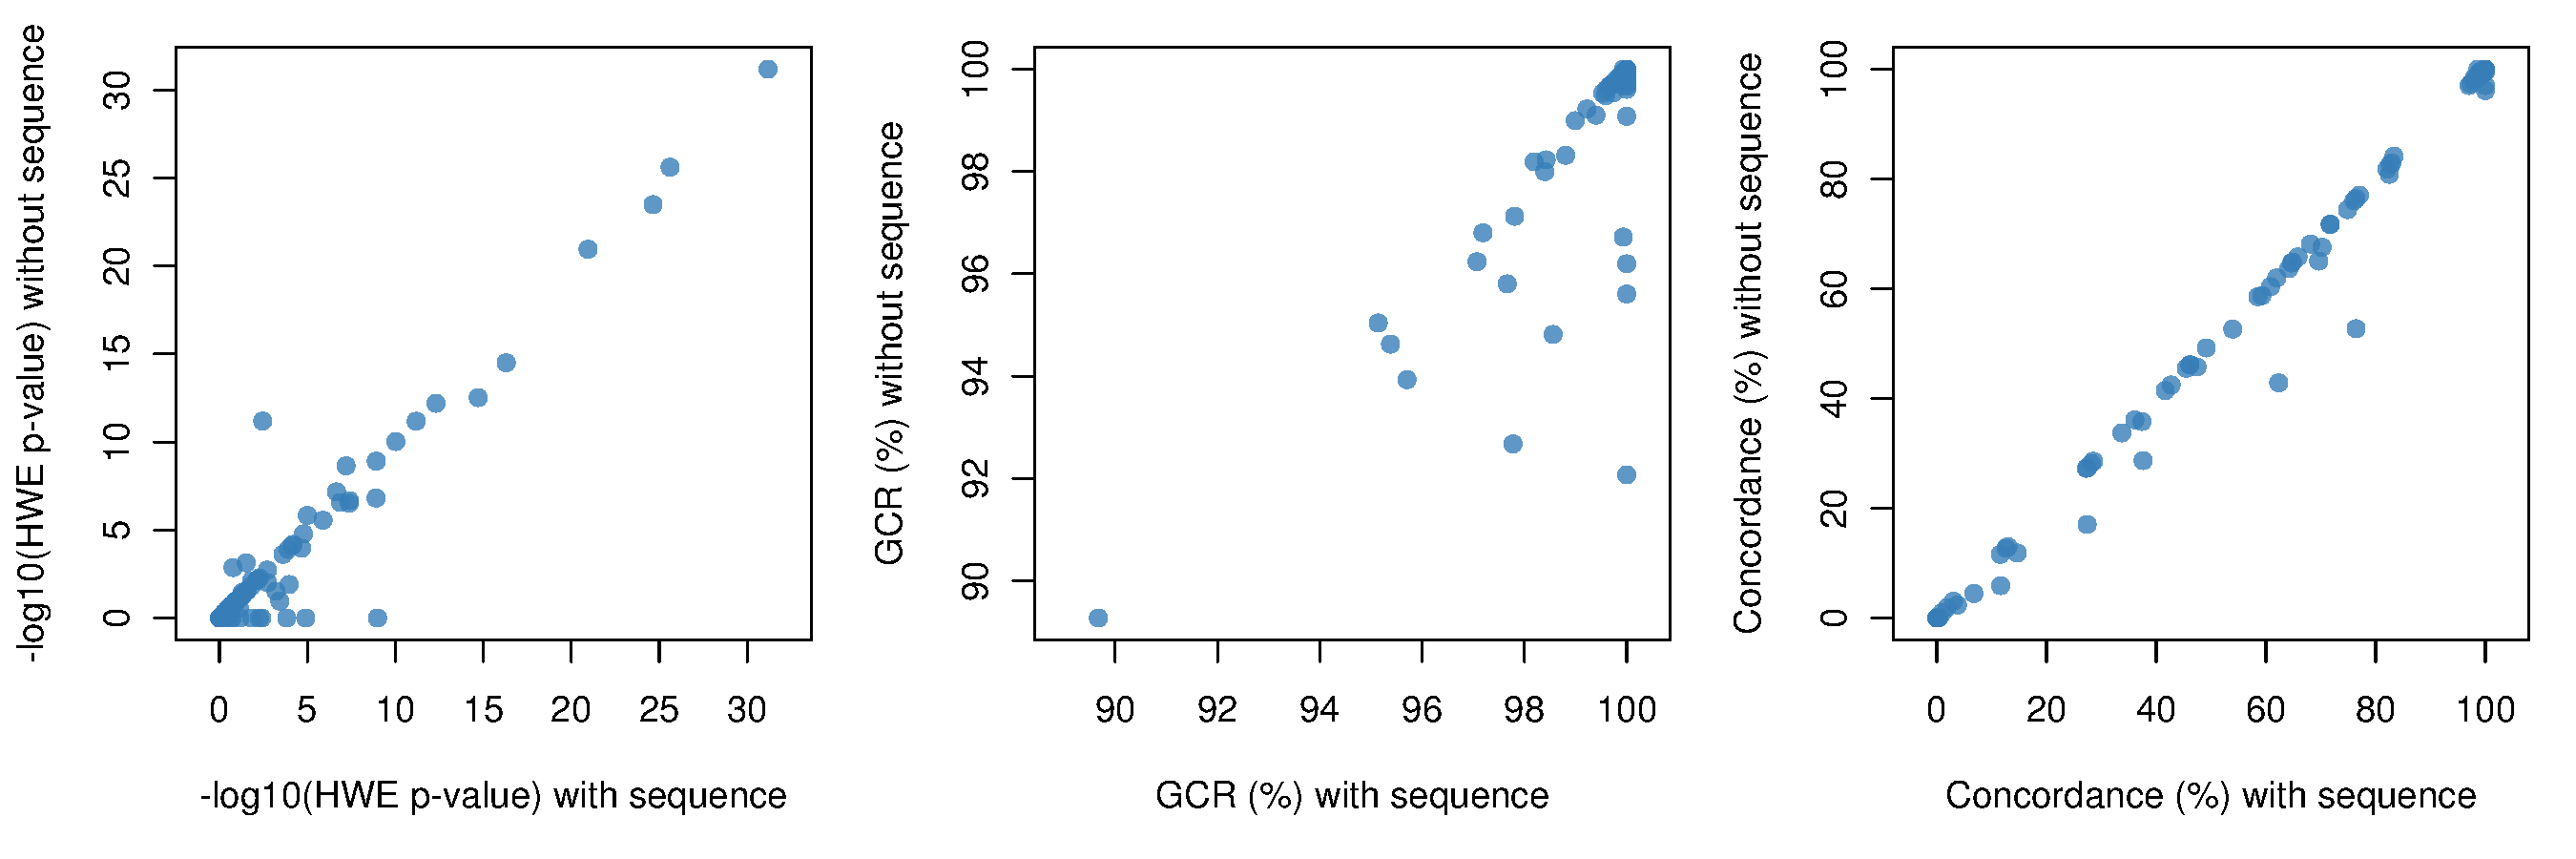
\includegraphics[width=\textwidth]{chap2figs/SupFig10}
    \caption[Evaluation of genotype calling when sequence data is problematic]{Comparison of calling with (x-axes) and without (y-axes) the use of sequence data on the 33 SNPs on the Axiom chip with high sequence failure rate, $\eta_Y > 0.5$. Left :  $-\log_10$ p-value for HWE. Middle : GCR. Right : Concordance.
      \label{chap2:results:eta_seq} }
  \end{center} 
\end{figure}


\begin{figure}[p]
  \begin{center} 
    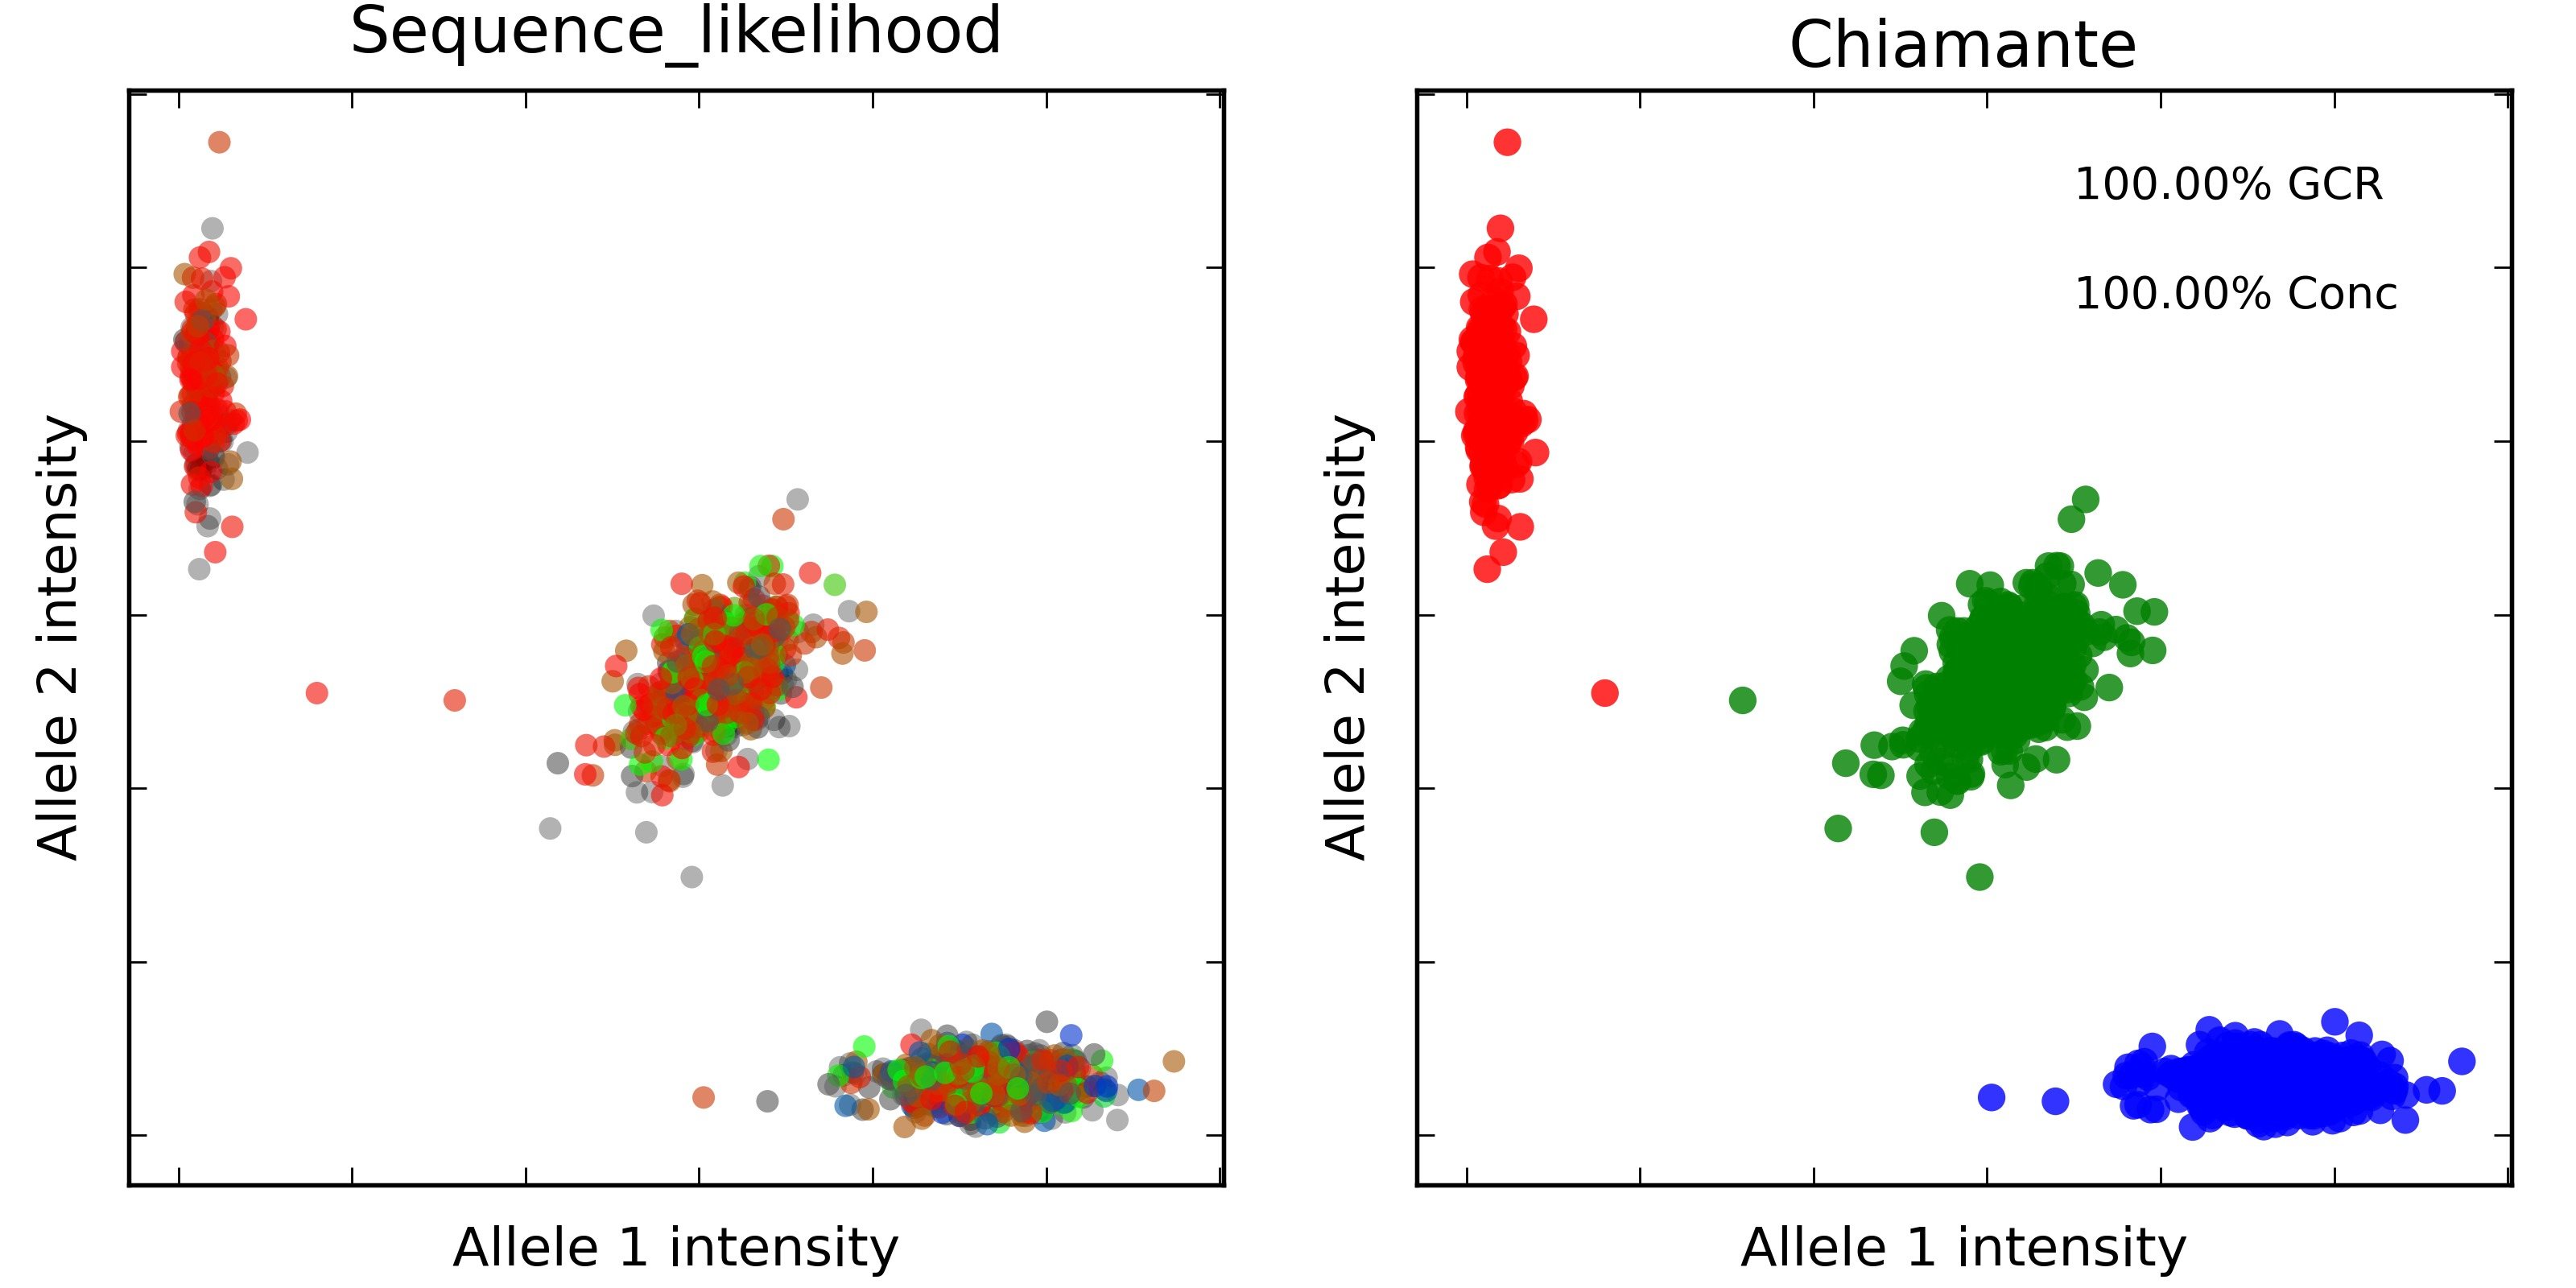
\includegraphics[width=\textwidth]{chap2figs/Fig5}
    \caption[Illustration of a SNP with high estimated sequence failure]{Illustration of a SNP with high estimated failure rate for the sequence assay ($\eta_Y = 0.63$). The left plot shows the cluster plot for the SNP with points coloured using a RGB colour scheme based on the scaled GLs for each genotype. The right hand plots shows the same cluster plot with points coloured according to the Chiamante posterior probabilities.\label{seq_fail_1}}
  \end{center} 
\end{figure}



\begin{figure}[p]
  \begin{center} 
    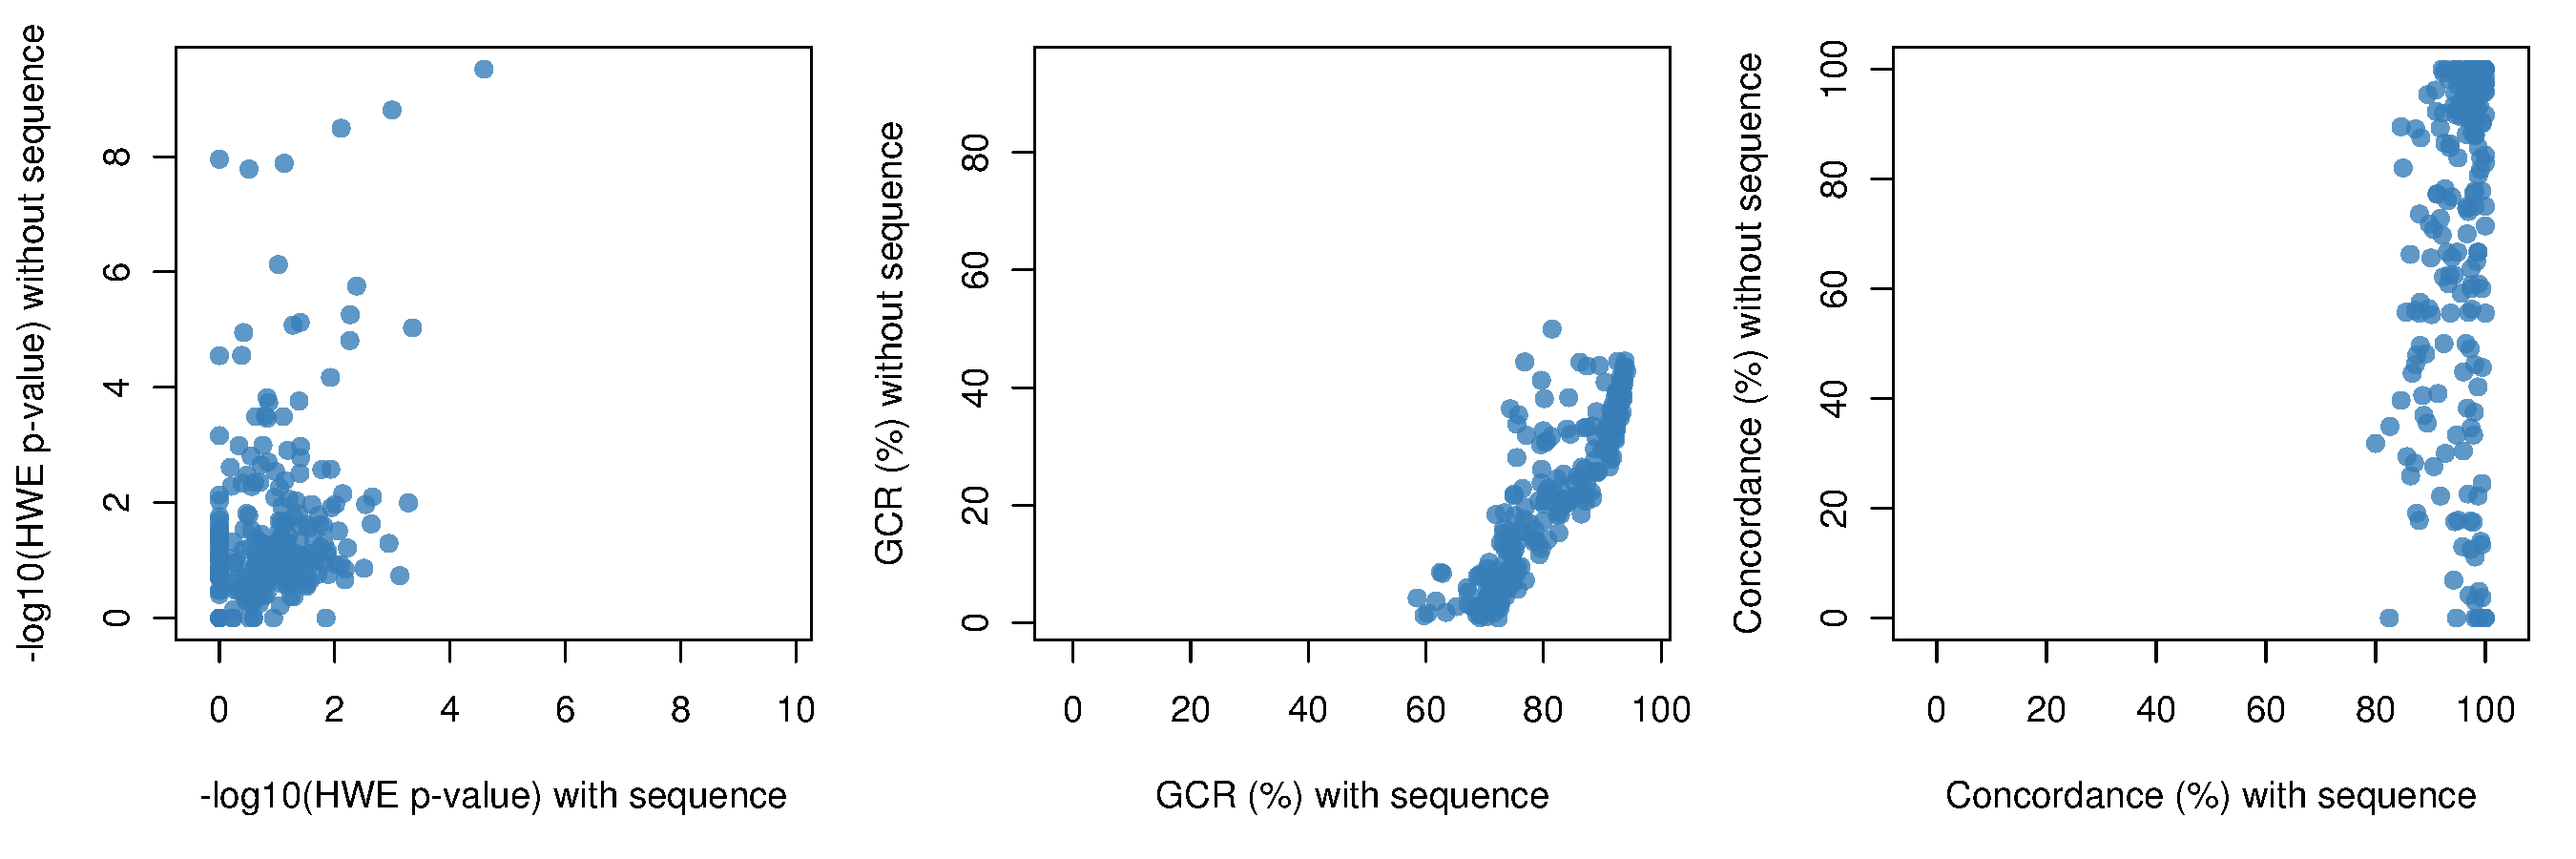
\includegraphics[width=\textwidth]{chap2figs/SupFig11}
    \caption[Evaluation of genotype calling when array data is problematic]{Comparison of metrics on the 235 SNPs called with high array failure rate, $\eta_X> 0.5$ . Plots of $-\log_{10}(\textrm{HWE p-value})$ (top), GCR (middle) and concordance (bottom) on these SNPs called with and without the use of sequence data.
      \label{chap2:results:eta_array}}
  \end{center} 
\end{figure}

\begin{figure}[p]
  \begin{center} 
    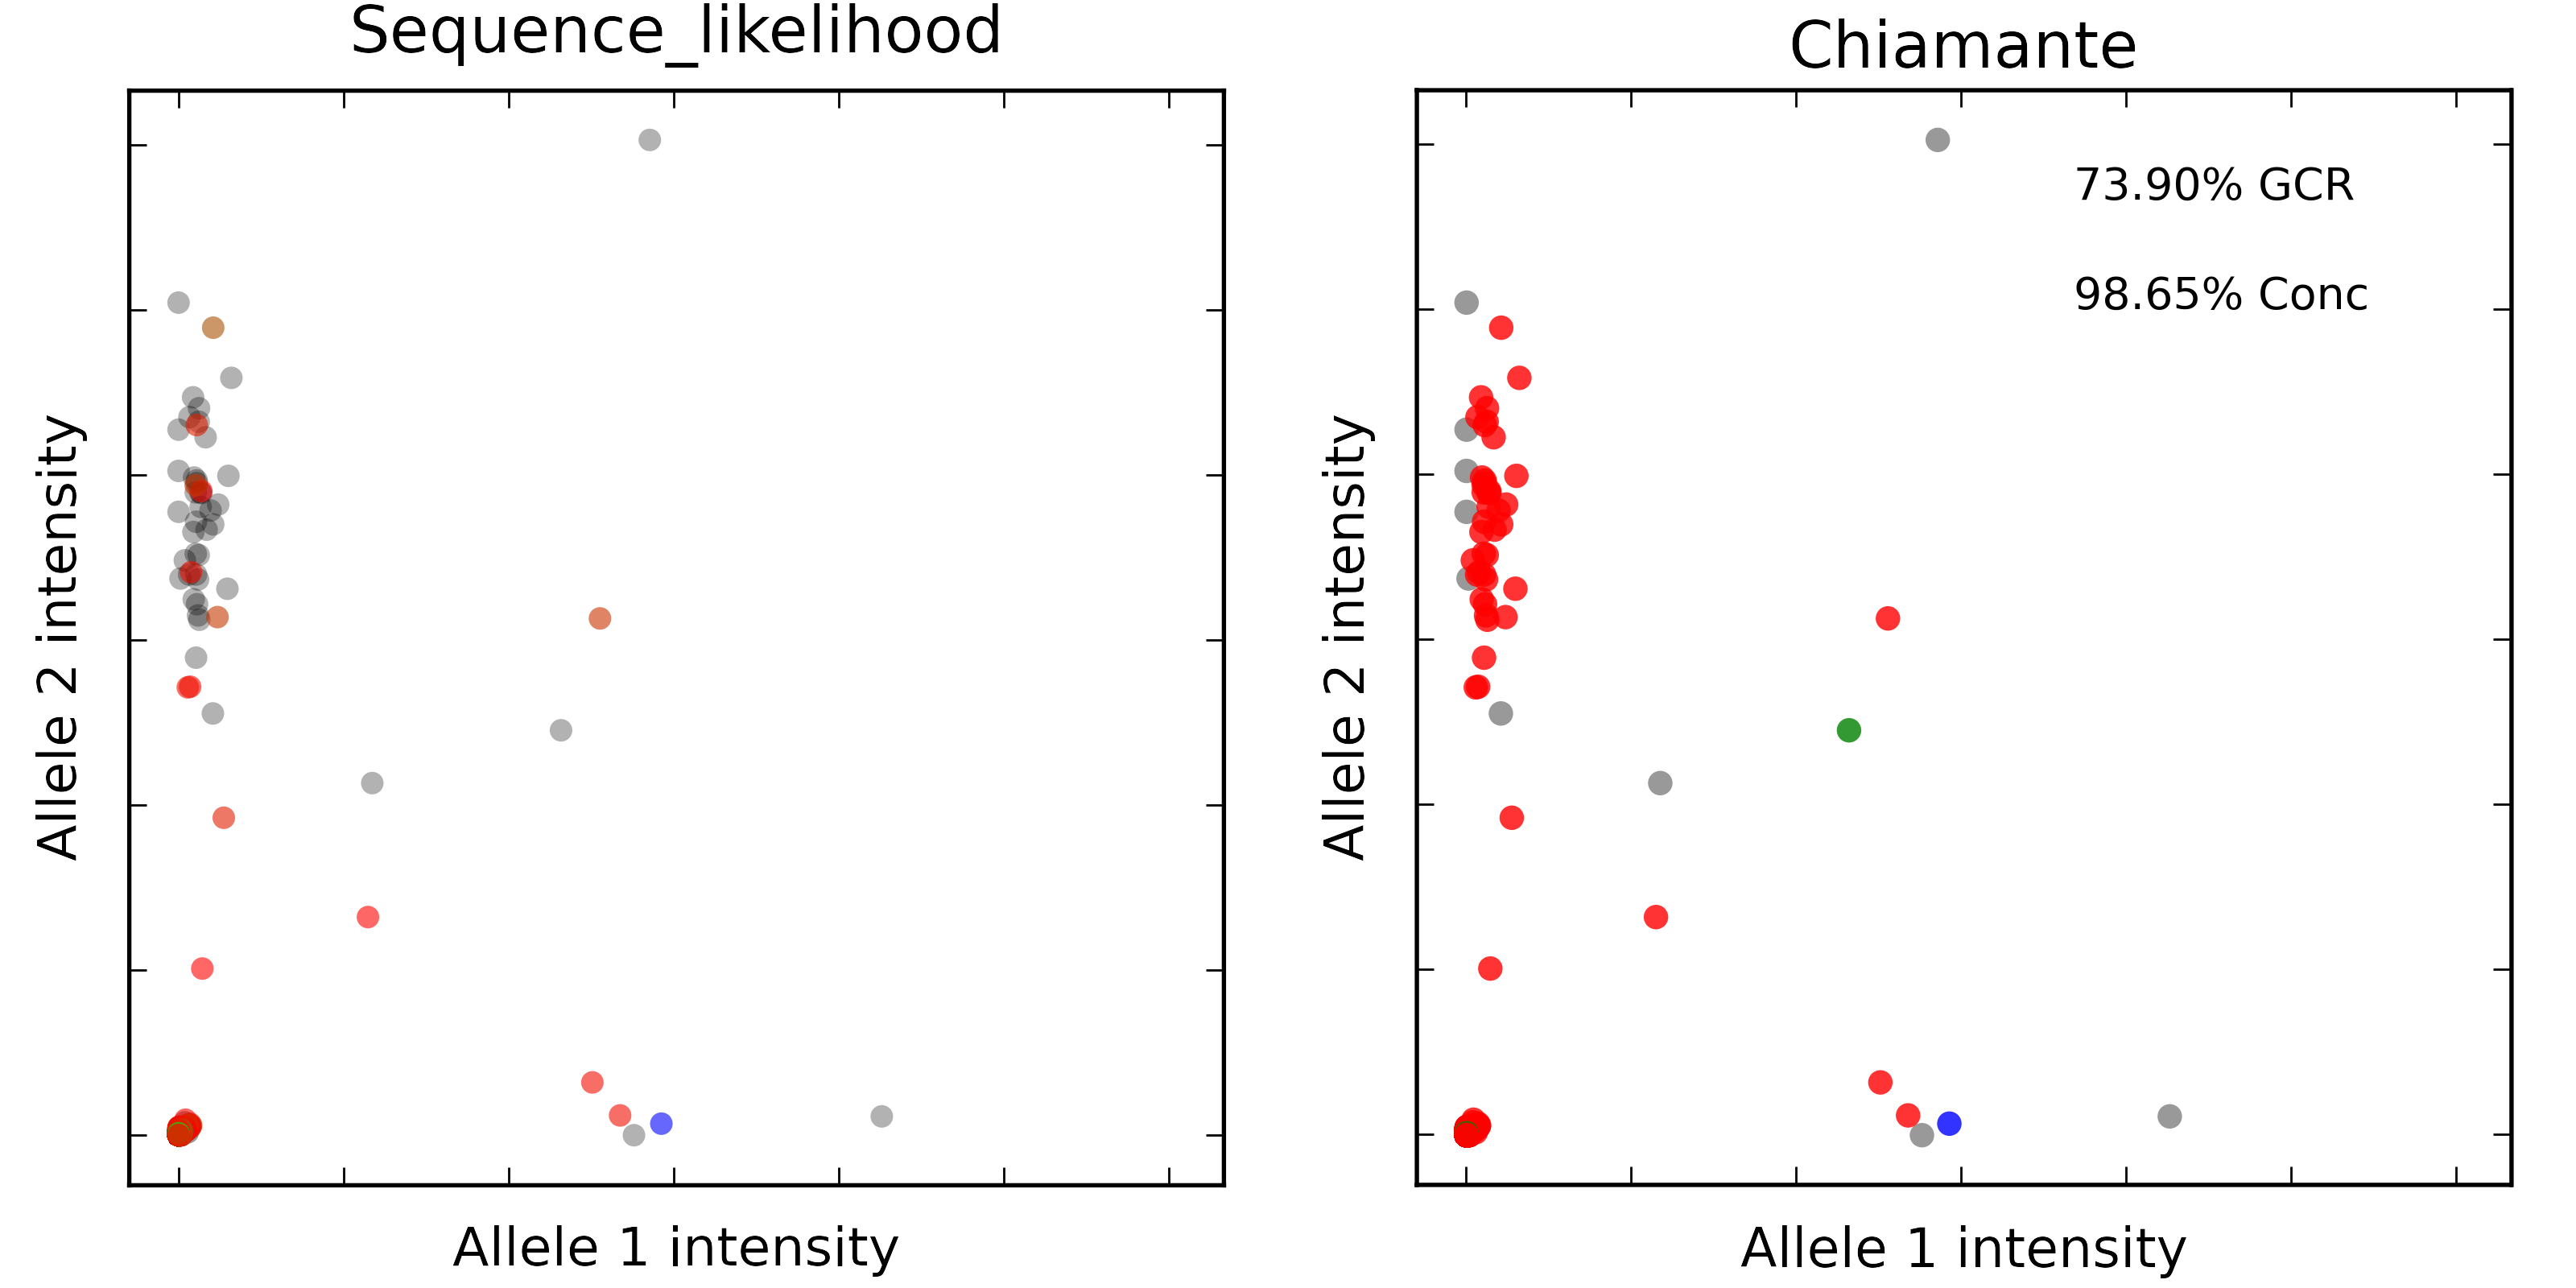
\includegraphics[width=\textwidth]{chap2figs/arrayfail_snp}
    \caption[Illustration of a SNP with high estimated array failure]{Illustration of a SNP with high estimated failure rate for the array assay ($\eta_X=0.71$). The left plot shows the cluster plot for the SNP with points coloured using a RGB colour scheme based on the scaled GLs for each genotype. The right hand plots shows the same cluster plot with points coloured according to the Chiamante posterior probabilities.   \label{array_fail_1}}
  \end{center} 
\end{figure}

\section{Discussion}

In this chapter we have introduced a genotype calling method for micro-array data that can leverage additional information from sequenced individuals and compared this model to other state of the art techniques.  As a traditional ``array only'' calling routine it is competitive with Illumina's proprietary software, achieving similar call rate and accuracy and substantially better that Illuminus and GenoSNP.  The addition of sequencing data makes our method the most accurate across a range of scenarios, although only by a modest margin.  This allows a greater number of SNPs (1000s) to pass standard QC filters.  The gains at low frequency sites were more substantial than common sites.  The failure indicators of the model also show potential as useful QC parameters.

An important limitation to note with this model is that it can identify when one of the assays has failed, but not both. Since we have reasonably realistic distribution for the failure mode of microarray data, observations that fit this failure distribution better than any of the genotype clusters can be flagged as uninformative and the sequence likelihoods are used.  However, sequence failures can only be identified when the GLs are strongly discordant with the information from microarrays. Hence in the case of very poor quality microarray data \emph{and} poor quality sequence data, the sequence data will not be flagged as erroneous.  In practice it would be prudent to filter SNPs where either assay has a high failure rate.

The model we have proposed may not capture the full complexity of imperfect sequence and array data. Our model assumes that assays have either succeeded or failed but they may include partial information. For example, errors in some reads covering a SNP site might contain sequencing errors or mapping errors that we do not model explicitly. To a certain extent the use of genotype likelihoods accounts for some of these error modes. Also, we have assumed errors are independent but errors could be correlated due to local sequence features such as GC content or proximity of SNPs to short insertions and deletions. 

Despite these limitations, the model performs well in general and even in the very extreme scenarios such as those shown in Figures~\ref{array_fail_1}~and~\ref{seq_fail_1}.  The gains we make are modest,  this is perhaps not surprising given that Illumina's standard software calls 99.72\% of genotypes with 99.71\% accuracy which is a testament to the high quality of the current generation of micro-array data.  Nevertheless, the computation required for our method is not substantial (< 1 day for the data set described here) and there is always a case for producing the most accurate set of genotypes as possible.



